
\documentclass[a4paper,11.5pt]{report} 
\usepackage{graphicx}
\usepackage{url}
\usepackage[utf8]{inputenc}
\usepackage[small,bf,hang]{caption2}
\usepackage{xspace}
\usepackage{graphicx}
\usepackage{fixltx2e}
\usepackage{amsmath}
\usepackage{float}
\usepackage{tikz}
\usepackage{amsmath}

\graphicspath{ {afb/} }

\newcommand{\HRule}{\rule{\linewidth}{0.5mm}}

\begin{document}

\pagenumbering{arabic}

% Geef hierna je titel, naam en de datum in,
% de titelpagina wordt automatisch aangemaakt.
%\title{Ingenieursproject II}

%\author{Jan Janssens\\jan@jansenss.be}
%\date{25 november 2004}
%\maketitle

\begin{titlepage}
\begin{center}

% Upper part of the page. The '~' is needed because \\
% only works if a paragraph has started.

\includegraphics[width=\linewidth]{ugent}~\\[2.5cm]

\textsc{Project in het kader van het Vakoverschrijdend Projectvak in de Bachelor Computerwetenschappen}\\[1.5cm]



% Title

{ \huge \bfseries Triump \\[0.4cm] }

\HRule \\[1.5cm]

% Author and supervisor
\begin{minipage}{0.5\textwidth}
\begin{center} \large
\emph{Groep 2}\\
Siebe \textsc{Claes}\\
Vincent \textsc{Dutordoir}\\
Lars \textsc{Hulstaert}\\
Jonas \textsc{Spanoghe}\\[2.5cm]
\emph{Titularis}\\
prof.~dr.~ir.~ Dirk \textsc{Stroobandt}\\[0.2cm]
\emph{Promotor}\\
prof.~dr.~ir.~ Bart \textsc{dhoedt}\\[0.2cm]
\emph{Begeleiders}\\
dr.~ir. Tim \textsc{Verbelen}\\
dr.~ir. Bert \textsc{Vankeirsbilck}\\
\end{center}
\end{minipage}

\vfill

% Bottom of the page
{\large Academiejaar 2014 - 2015}

\end{center}
\end{titlepage}

\tableofcontents

\chapter{Inleiding}

Sinds de opgang van smartphones in 2006 zijn reeds 1.2 miljard toestellen verkocht\cite{smartphone_sales}. 28 \% van het gebruik van smartphones wordt vandaag gelinkt aan sociale media. Locatie-gebaseerde applicaties zoals Foursquare\cite{foursquare} en Swarm\cite{swarm} zijn een nieuwe vorm van sociale media, voortstuwend op de opmars van smartphones, waarbij gebruikers hun locatie kunnen delen met hun vrienden.
Sociale media trekken een enorm publiek aan en vormen zo een ideale doelgroep voor online marketing.\\

In dit vakoverschrijdend project wordt een toepassing ontwikkeld die ernaar streeft om sociale media te integreren met lokale bedrijven.
De applicatie vormt voor gebruikers een sociaal platform, terwijl bedrijven het als online marketing tool kunnen inzetten.\\

In de volgende sectie wordt de probleemstelling verder uitgediept. In het derde onderdeel worden functionele en niet-functionele vereisten opgesteld. Vervolgens wordt besproken hoe het project technisch opgebouwd is, zowel op vlak van architectuur als specifiek ontwerp. In de sectie resultaten wordt de eigenlijke applicatie besproken, en teruggekeken naar de functionele en niet-functionele vereisten. Hierna wordt een overzicht gegeven van de planning en samenwerking gedurende het project. In de laatste sectie van het verslag worden de openstaande problemen geanalyseerd.
\chapter{Probleemstelling}
Om tot het idee van dit project te komen hebben we eerst bestaande locatie-gebaseerde toepassingen en online marketing tools geanalyseerd. Vervolgens hebben we beide concepten gecombineerd in één applicatie, nl. Triump.

Vandaag bestaan reeds verschillende locatie-gebaseerde applicaties waarmee gebruikers hun huidige locatie kunnen delen met hun vrienden. 
De bekendste voorbeelden hiervan zijn Foursquare\cite{foursquare} en Swarm\cite{swarm}.
Foursquare is een sociale netwerksite die gebruikers plaatsen laat categoriseren en beoordelen.
Het is een mobiele applicatie waarmee men hippe locaties met elkaar kan delen. Met Swarm daarentegen kunnen gebruikers `inchecken' op plaatsen en hun locatie delen met andere gebruikers. Swarm is een mobiele applicatie, die gebruik maakt van de Foursquare's locatiedatabase. Swarm is eerder gericht op het delen van locatieupdates in plaats van ervaringen en tips zoals het geval bij Foursquare.
Hoewel Swarm en Foursquare beide gericht zijn op het sociaal gebeuren, wordt er geen nadruk gelegd op het `samenbrengen' van mensen. 

Daarnaast onderzochten we ook online marketing platformen. Momenteel gebeurt online marketing voornamelijk op een manier die door gebruikers als intrusief en ongewenst ervaren wordt via online advertenties. Qustomer\cite{qustomer} daarentegen is een online marketing tool die erin is geslaagd om naast advertising ook iets extra aan gebruikers te bieden. Qustomer biedt gebruikers een klantenkaart in de vorm van een applicatie op de mobiele telefoon. Deze klantenkaart kan door verschillende ondernemingen gebruikt worden. Net zoals bij traditionele klantenkaarten, kan een gebruiker punten opsparen en hiermee promoties verkrijgen. Qustomer en andere van deze platformen staan los van enige vorm van sociale media, en bijgevolg is de aantrekkingskracht naar gebruikers toe eerder beperkt.

Vandaag bestaan beide media, locatie-gebaseerde sociale applicaties en online marketing tools, volledig onafhankelijk van elkaar en zijn er geen toepassingen die beide concepten combineren. 
Promoties vormen een stimulans om mensen gebruik te laten maken van de diensten van een bedrijf. Indien de promoties gericht zijn op groepen mensen en volgens het Groupon-principe werken, kunnen promoties een middel zijn om mensen samen te brengen.
In het Groupon-principe verkrijgt men namelijk voordelen door in grote groep diensten aan te kopen.
Afgelopen jaar Foursquare heeft 45 miljoen actieve gebruikers bereikt, en dat aantal is nog steeds aan het groeien. \cite{users}. Foursquare is dus een platform met het potentieel om een enorm publiek te bereiken wegens zijn functie als sociaal netwerk. 

Indien men concepten zoals Foursquare en Qustomer combineert, krijgt men een platform waarbij men mensen stimuleert om samen te komen omwille van promoties en men deze bereikt via Foursquare.
Triump is een mobiele applicatie met als doel beide te koppelen.
Concreet breidt Triump de functionaliteit van Foursquare uit en wordt het marketing aspect gebaseerd op het concept van Qustomer.



\chapter{Doelstelling}

De doelstelling van deze Bachelorproef is het ontwikkelen van een locatie-gebaseerde sociale applicatie, die tevens dienst doet als online marketing tool, genaamd Triump. Als onderdeel van de objectgeoriënteerde analyse worden de functionele en niet-functionele vereisten meegegeven.
Concreet breiden we de functionaliteit uit van Swarm en Qustomer. Vernieuwend aan Triump is dat gebruikers groepen kunnen creëren en hiervan lid kunnen worden. Inchecken in een locatie gebeurt, naast de persoonlijke checkin, ook in naam van de groepen waarvan men lid is.  


Voor elke locatie wordt een rangschikking bijgehouden aan de hand van de checkins van de verschillende groepen. Conceptueel biedt de applicatie de gebruikers een platform om in groep `king of the hill' te spelen. Het principe van `king of the hill' is dat er 1 gebruiker of groep als `koning' bovenaan de heuvel staat en dat andere groepen de heuvel proberen te veroveren om zo zelf koning te worden. Bij Triump kunnen gebruikers lid worden van groepen, en in groepsverband inchecken. Hierdoor stijgen de groepen in de ranglijst van de locatie. Een locatie wordt veroverd door de groep die bovenaan de ranglijst staat.
Bij Triump is er dus 1 groep of `koning' die voor een locatie bovenaan de ranglijst staat.

Los van het competitief karakter van deze applicatie (bv. verschillende studentenverenigingen die strijden om het ‘bezit’ van locaties in een studentenstad) kan deze applicatie ook ingezet worden als marketing tool, en dus de functionaliteit van Qustomer integreren.
Triump biedt lokale ondernemingen namelijk de mogelijkheid om evenementen te organiseren. Aan een evenement kan men dan een begin- en eindstip, en een promotie toekennen. Gebruikers die bijvoorbeeld na een week aan de top van een locatie staan of m.a.w. het meeste ingecheckt hebben kunnen nadien beloond worden met een promotie. Daarnaast kunnen ook gewone gebruikers evenementen organiseren en deze koppelen aan een bepaalde locatie.
Enerzijds zijn er dus de evenementen die gebruikers voor hun vrienden organiseren waarvan de zichtbaarheid beperkt is tot een aantal groepen. Anderzijds zijn er de `officiële' evenementen waarbij promoties kunnen gewonnen worden die zichtbaar zijn zijn voor alle gebruikers. 
\\Concreet is Triump dus een sociaal spel waarbij men in groepsverband populaire locaties kan innemen en aan evenementen kan deelnemen.

\section{Niet-functionele vereisten}
De niet-functionele vereisten stellen de kwaliteitseisen voor waaraan het project moet voldoen. Hiervoor focussen we ons voornamelijk op gebruiksvriendelijkheid, configureerbaarheid, robuustheid, schaalbaarheid en beschikbaarheid.
Gebruiksvriendelijkheid en configureerbaarheid situeren zich op niveau van de applicatie (frontend). Voor mobiele applicaties is het belangrijk dat de applicatie intuïtief is en gemakkelijk in gebruik. Een belangrijk onderdeel van het ontwerp is het uitdenken van een gebruiksvriendelijke user interface. Configureerbaarheid is ook een belangrijk aspect. Triump zal gebruikt worden als marketing tool, en hierbij moet de gebruiker zelf kunnen beslissen hoe hij/zij hiermee in aanraking komt. Notificaties over nieuwe promoties moeten bijvoorbeeld uitgeschakeld kunnen worden indien de gebruiker hiervan niet op de hoogte wil gebracht worden. Daarnaast gaat de voorkeur uit naar een mobiele applicatie die de gebruiker naar wens kan personaliseren.
Robuustheid, schaalbaarheid en beschikbaarheid situeren zich op niveau van de backend. Deze aspecten van het ontwerp zijn, hoewel niet zichtbaar voor de gebruiker, essentieel voor een aangenaam en continu gebruik van de applicatie.
\\\\
\section{Functionele vereisten}
De functionele vereisten worden opgesplitst in twee delen. Enerzijds zijn er de algemene acties die de basis vormen van Triump en anderzijds zijn er de acties die de gebruiksvriendelijkheid van de applicatie bevorderen. Onderstaande oplijsting geeft heel concreet en beknopt weer wat een gebruiker kan doen met Triump.

\begin{itemize}
	
\subsubsection{Algemeen}
\item Inloggen op de applicatie via een Foursquare account.
\item Beheren van een groep: aanmaken van een groep door naam, beschrijving en type op te geven, accepteren van nieuwe leden en verwijderen van leden.   
\item Bekijken van alle groepen en op een eenvoudige manier een groep kunnen zoeken.
\item Lidverzoek versturen naar een groep.
\item Bekijken van alle leden van een groep.
\item Bekijken van een profiel van een gebruiker.
\item Bekijken van alle locaties en op eenvoudige manier een locatie kunnen zoeken.
\item Inchecken op een locatie. Daarbij wordt de checkin doorgepropageerd naar Foursquare. De checkin telt mee voor elke groep waartoe de gebruiker behoort. 
\item Bekijken van de ranglijst van een locatie.
\item Aanmaken van een evenement op een locatie. Een gebruiker kan een naam, beschrijving, beloning, start- en eindtijdstip opgeven en groepen uitnodigen.
\item Bekijken van alle evenementen waartoe de gebruiker is uitgenodigd.
\item Bekijken van de ranglijst van een evenement.
\item Aanmaken van een officieel evenement. Dit evenement moet zichtbaar zijn voor alle gebruikers.
\item Bekijken van alle gewonnen evenementen en de bijhorende promotie ophalen.

\subsubsection{Gebruiksvriendelijkheid}

\item Gebruiker ontvangt notificaties van belangrijke gebeurtenissen.
\item Wijzigen van instellingen en privacybeleid. Een gebruiker kan de zichtbaarheid van zijn/haar profiel beperken. Een gebruiker kan notificaties in- of uitschakelen. Een gebruiker kan ook het uiterlijk van de applicatie configureren naar eigen smaak.
\item Gebruiker kan zijn/haar feedback  op een eenvoudige manier doorgeven via de applicatie.

\end{itemize}


% Laten vallen
%\chapter{}

%Een beschrijving van de opdeling van het project in deeltaken en de
% taakverdeling over de groepsleden.



\chapter{Planning en taakverdeling}

% De initieel opgemaakte planning en de uiteindelijke uitvoering (in Ganttchart-achtige
% vorm) met een korte verklaring van de verschillen.

\subsubsection{Initiele planning}

Figuur \ref{fig:planning_initieel} in de bijlagen toont de initiële planning. De planning werd opgesteld naar aanleiding van de eerste presentatie en is bijgevolg relatief vaag. Desalniettemin is het hoofdprincipe van deze initiële planning doorheen het volledige project blijven gelden. 

Het prinicipe weergegeven in figuur \ref{fig:planning_initieel} is de gelaagde opbouw van Triump. Er wordt namelijk met drie "cores" gewerkt. De eerste core van de drie cores bevat de absolute basis van de applicatie zoals communicatie met de backend, een basis-activiteit die de locatie van een gebruiker bepaald en een login en logout scherm. In de tweede core worden de basisonderdelen van Triump zoals locaties, events, rewards, groepen, gebruikers en een basis UI geïntegreerd in de applicatie. Een laatste core richt zich voornamelijk op gebruiksvriendelijkheid en afwerking. In deze core bevinden zich elementen zoals een notificatiesysteem, instellingenpagina, feedbacksysteem en een aantrijkelijke UI. Het was de bedoeling de core gelijktijdig op de backend en de frontend te implementeren.

Na het uitwerken van de kern werd tijd voorzien voor uitbreidingen. Mogelijk uitbreidingen waren: het voorzien korte spelletjes om op een tweede manier punten te kunnen verdienen, iOS of WindowsPhone versie en een integratie met Qustomer. 

De laatste weken van het project gingen voornamelijk gebruikt worden om het verslag te schrijven en als voorbereiding voor de eindpresentatie.

\subsubsection{Uiteindelijke planning en verschillen met initiële planning}

Figuur \ref{fig:planning_initieel} in de bijlagen toont de uiteindelijke planning. In bovenstaande paragraaf werd reeds aangehaald dat Triump opgebouwd is uit meerdere kernen, in deze planning werd elk onderdeel van deze kernen uitgewerkt teneinde een gedetailleerd overzicht te geven van de gevolgde werkwijze. Het grootste verschil met de initiële planning is de toevoeging van de webinterface. De nood van een webinterface was gedurende de opstelling van de eerste planning niet gekend. Bijgevolg was het noodzakelijk de tijd nodig voor het bouwen van de webinterface te voorzien in de planning. 
De figuur toont ook aan dat er geen uitbreidingen geïmplementeerd zijn dit is voornamelijk te wijten aan de bijkomende taak en de opgelopen vertraging tijdens de ontwikkeling van core 2.

\subsubsection{Taakverdeling}

Figuur \ref{fig:planning_initieel} geeft naast de planning ook de taakverdeling weer. Meermaals per week werd er met alle leden samen gekomen om het project te evalueren en de taken te verdelen. De taken werden zo verdeeld dat elk groepslid zowel aan de frontend als aan de backend gewerkt heeft.


\chapter{Architectuur}

Het technische aspect van Triump bestaat uit twee grote delen. Enerzijds is er de frontend, waarmee de gebruikers rechtstreeks interageren, en anderzijds is er de backend, verborgen voor iedere gebruiker. De frontend bestaat op zijn beurt uit twee delen, nl. een Android applicatie en een webinterface. De backend is ontwikkeld op Google Cloud Endpoints. In figuur \ref{fig:algemene structuur} wordt schematisch de structuur van Triump weergegeven. In dit hoofdstuk wordt er dieper ingegaan op de gebruikte technologieën van de verschillende onderdelen. In het volgend hoofdstuk wordt dan eerder gefocust op het specifiek ontwerp en implementatie van de verschillende onderdelen. Steeds wordt er een onderscheid gemaakt tussen technologieën gehanteerd in de backend of in de frontend.

%nieuwe figuur
\begin{figure}[H]
	\centering
	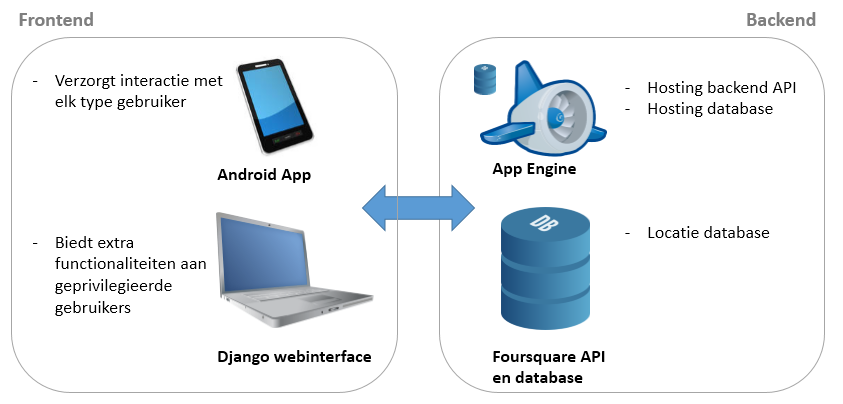
\includegraphics[scale=0.5]{achitectuur}
	\caption{Architectuur bestaat uit twee grote delen, enerzijds de backend en anderzijds de frontend. De backend bestaat uit een combinatie van een App Engine instantie en de Foursquare API. De frontend bestaat uit een Android app en een django webinterface.}
	\label{fig:algemene structuur}
	
\end{figure}

\section{Backend}

\subsection{Google Cloud Endpoints}
\label{sec: GCE}
Google Cloud Endpoints (GCE) is een uitbreiding van Google App Engine (GAE). GAE is een bekend 'Platform as a Service' ontworpen om applicaties uit te voeren op Googles infrastructuur. GCE biedt naast de functionaliteiten beschikbaar in GAE de mogelijkheid om op een relatief eenvoudige manier een backend API te genereren voor applicaties.  Endpoints verzorgt onder andere de communicatie en authenticatie tussen gebruikers en de backend.
Aangezien GCE nog steeds gehost wordt door een Googles App Engine instantie blijven alle andere functionaliteiten zoals 'Datastore' voor dataopslag, 'Google Cloud Messaging' voor notificaties en 'Cron Jobs' voor periodieke taken beschikbaar. Figuur \ref{fig:Overzicht Google Cloud Endpoints} geeft een overzicht van Google Cloud Endpoints weer~\cite{Google_endpoints}.

\begin{figure}[H]
	\centering
	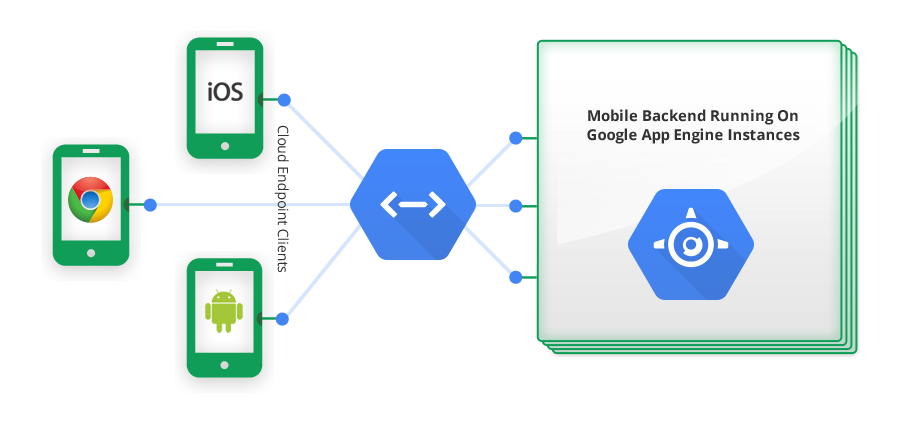
\includegraphics[scale=0.3]{GCE}
	\caption{De endpoints  bieden een gebruiksvriendelijke interface voor de functionaliteiten van Google App Engine.}
	\label{fig:Overzicht Google Cloud Endpoints}
\end{figure}

Het voornaamste voordeel van het werken met GAE is dat er tijdens ontwikkelfase geen rekening hoeft gehouden te worden met het  beheer en de administratie van de backend infrastructuur. Een probleem zoals schaalbaarheid wordt via dynamische rekenkrachtallocatie opgelost. Daarnaast is de backend van Triump ook altijd bereikbaar aangezien GAE een hoge graad van permanentie van zijn servers verzekert. Desalniettemin brengt het gebruik van GAE ook enkele nadelen met zich mee. De voornaamste zijn de restricties op het aantal lees- en schrijfoperaties per dag, de sterk variërende duratie van lees- en schrijfoperaties en de afhankelijkheid van een externe organisatie. De restricties op het aantal operaties zijn enkel aanwezig bij gratis gebruik van GAE en kunnen geremediëerd worden door te betalen voor de diensten van GAE.
Aangezien elke nieuwe ontwikkelaar \$ 300 in GAE krediet krijgt, kon dit probleem tijdens de ontwikkelfase opgelost worden door het aantal operaties per dag van 50.000 naar 1.000.000 te verhogen. Een groot aantal operaties is vereist omdat elke atomaire lees/schrijf operatie wordt meegerekend. Hierdoor neemt het aantal leesoperaties/schrijfoperaties bij het uitvoeren van enkele complexe operaties zeer snel toe. De duratie van operaties op de GAE kan beperkt worden door te investeren in snellere apparatuur (met GAE krediet). Hiervoor werd tijdens de ontwikkeling niet voor gekozen.

\subsubsection{Datastore~\cite{Google_Datastore}}

Triump maakt gebruik van App Engine Datastore als backend databank. GAE Datastore verschilt van traditionele relationele databases door zijn specifieke architectuur. De database is namelijk zo ontworpen dat deze automatisch meeschaalt met de toenemende hoeveelheid opgeslagen data. Een tweede verschil met relationele databanken is dat GAE Datastore schemaloos is. Data wordt in de Datastore opgeslagen als objecten. Objecten van een eenzelfde type hebben verschillende velden en per veld kunnen verschillende datatypes opgeslagen worden.
Aangezien de database schemaloos is en bijgevolg bijvoorbeeld geen types zal controleren of niet zal aangeven indien een vreemde sleutel niet bestaat ligt de verantwoordelijkheid van de integriteit van de database volledig bij de ontwikkelaar. Tijdens de ontwikkeling werd dit gezien als het grootste nadeel van de GAE Datastore tegenover een traditionele relationele database.

\subsubsection{Google Cloud Messaging~\cite{Google_Cloud_Messaging}}

Google Cloud Messaging (GCM) voor Android is een dienst die het mogelijk maakt data (tot 4kB) te versturen van backend servers naar Android applicaties onder de vorm van boodschappen. De GCM servers staan in voor de connectie naar het mobiele toestel en een correcte aflevering van de berichten. De ontvangen boodschappen kunnen na aflevering eenvoudig omgevormd worden tot een notificatie. GCM wordt daarom gebruikt als basistechnologië voor het notificatiesysteem in Triump.

\subsubsection{Cron jobs~\cite{Google_Cron_Jobs}}

Een van de functionaliteiten die Google App Engine aanbiedt is de App Engine Cron Service. Deze service laat gebruikers toe bepaalde taken (cron jobs/chronical jobs) op regelmatige tijdstippen uit te laten voeren op de backend.


\subsection{Foursquare API}
\label{Foursquare API}
Triump is een locatie-gebaseerde applicatie. De locaties worden bekomen via de Foursquare API en locatiedatabase \cite{FS_API_website}. Naast locatie gegevens kan er ook informatie van gebruikers zoals namen, geboortedata en profielfoto's opgevraagd worden.
Het grote voordeel van de Foursquare API is dat locatiedata niet door de gebruikers zelf moet gegeneerd worden. Bovendien komt Triump, door deel van de functionaliteit van Swarm en Foursquare over te nemen, bij de gebruikers als vertrouwd over; een deel van de bestaande userbase kan overgenomen worden. 
Het gebruikte mechanisme in de Foursquare API is zeer vanzelfsprekend. Alle gegevens, opgeslaan in de database, zijn benaderbaar via een RESTful (Representational State Transfer) URL (Uniform Resource Locator) . De frontend applicatie dient een connectie over HTTPS te starten met een Foursquare API Endpoint via de gewenste URL. Vervolgens zal de API Endpoint de gevraagde informatie in JSON (Javascript Object Notation) formaat terugzenden. JSON is een gestandaardiseerd gegevensformaat.
Het werken met de API brengt echter wel enkele nadelen met zich mee.
Allereerst wordt Triump hierdoor opnieuw afhankelijk van een externe organisatie (naast Google). Indien Foursquare beslist zijn open database te sluiten moet het ontwerp van Triump volledig herzien worden. Daarnaast wordt van commerciële applicaties verwacht dat ze reclame maken voor Foursquare door bijvoorbeeld het Foursquare logo op te nemen in de layout.  Een tweede nadeel is dat de dataopslag verdeeld wordt over twee databases. Enerzijds de Google Cloud Datastore waar de data over groepen en checkins worden bijgehouden en anderzijds de Foursquare Datastore waar de locatie en gebruikergegevens zijn opgeslaan. Een laatste nadeel is dat locaties verplicht geregistreerd moeten zijn bij Foursquare teneinde zichtbaar te zijn op Triump. 
Indien locaties intern zouden aangemaakt en opgeslagen worden zouden de eerste twee nadelen verholpen zijn. Deze voor de hand liggende oplossing wordt echter niet toegepast aangezien dit zou impliceren dat Triump vanaf nul zijn locatiedatabase zou moeten aanvullen. Hierdoor zouden gebruikers ontmoedigd worden Triump boven Foursquare te kiezen. Daarnaast propageert Triump een checkin door naar Foursquare waardoor we de functionaliteiten ervan uitbreiden. 
Het laatste probleem wordt opgelost door het voorzien van een webinterface. Deze interface voorziet de mogelijkheid aan eigenaars om locaties te registreren. Meer uitleg over de website volgt in de onderstaande paragraaf Webinterface.
\section{Frontend}
\subsection{Android applicatie}
\subsubsection{Waarom Android?}

Bij de ontwikkeling van de Triump applicatie is er gekozen voor Android als mobiel platform boven iOS of Windows Phone. Android heeft als voordeel dat het een groot marktaandeel heeft (76.6\% van de smartphones wereldwijd draait op Android \cite{marketshare}) en er dus een groot publiek bereikt kan worden met de applicatie. Dit maakt dat Android als eerste platform de beste keuze is. De ontwikkeltools voor iOS en Windows Phone zijn bovendien niet cross-platform. Om apps te ontwikkelen voor iOS dient men over XCode te beschikken (enkel beschikbaar op Mac OS X) en om Windows Phone applicaties te ontwikkelen maakt men gebruik van Visual Studio (enkel beschikbaar op Windows). Vermits het team bestaat uit 1 Windows, 1 Linux en 2 Mac gebruikers, was het noodzakelijk om een cross-platform ontwikkelomgeving te hebben.
\subsubsection{Ontwikkelomgeving: Android Studio}
% vergelijking vs Eclipse
Vroeger was Eclipse de standaard ontwikkelomgeving (IDE) voor Android. Hierbij werd de standaard Eclipse installatie uitgebreid met de Android Developer Toolkit (ADT) plugin om Eclipse beter geschikt te maken voor Android Development. Op 16 mei 2013 stelde Google de nieuwste IDE voor Android voor genaamd Android Studio. Deze IDE is gebaseerd op IntelliJ IDEA en biedt veel verbeteringen ten opzichte van Eclipse. 
De voordelen van Android Studio zijn legio: betere code generatie en auto-complete dan Eclipse, zeer goede integratie met de Android SDK en live previews in de layout builder. 

%\begin{figure}[H]
%	\centering
%	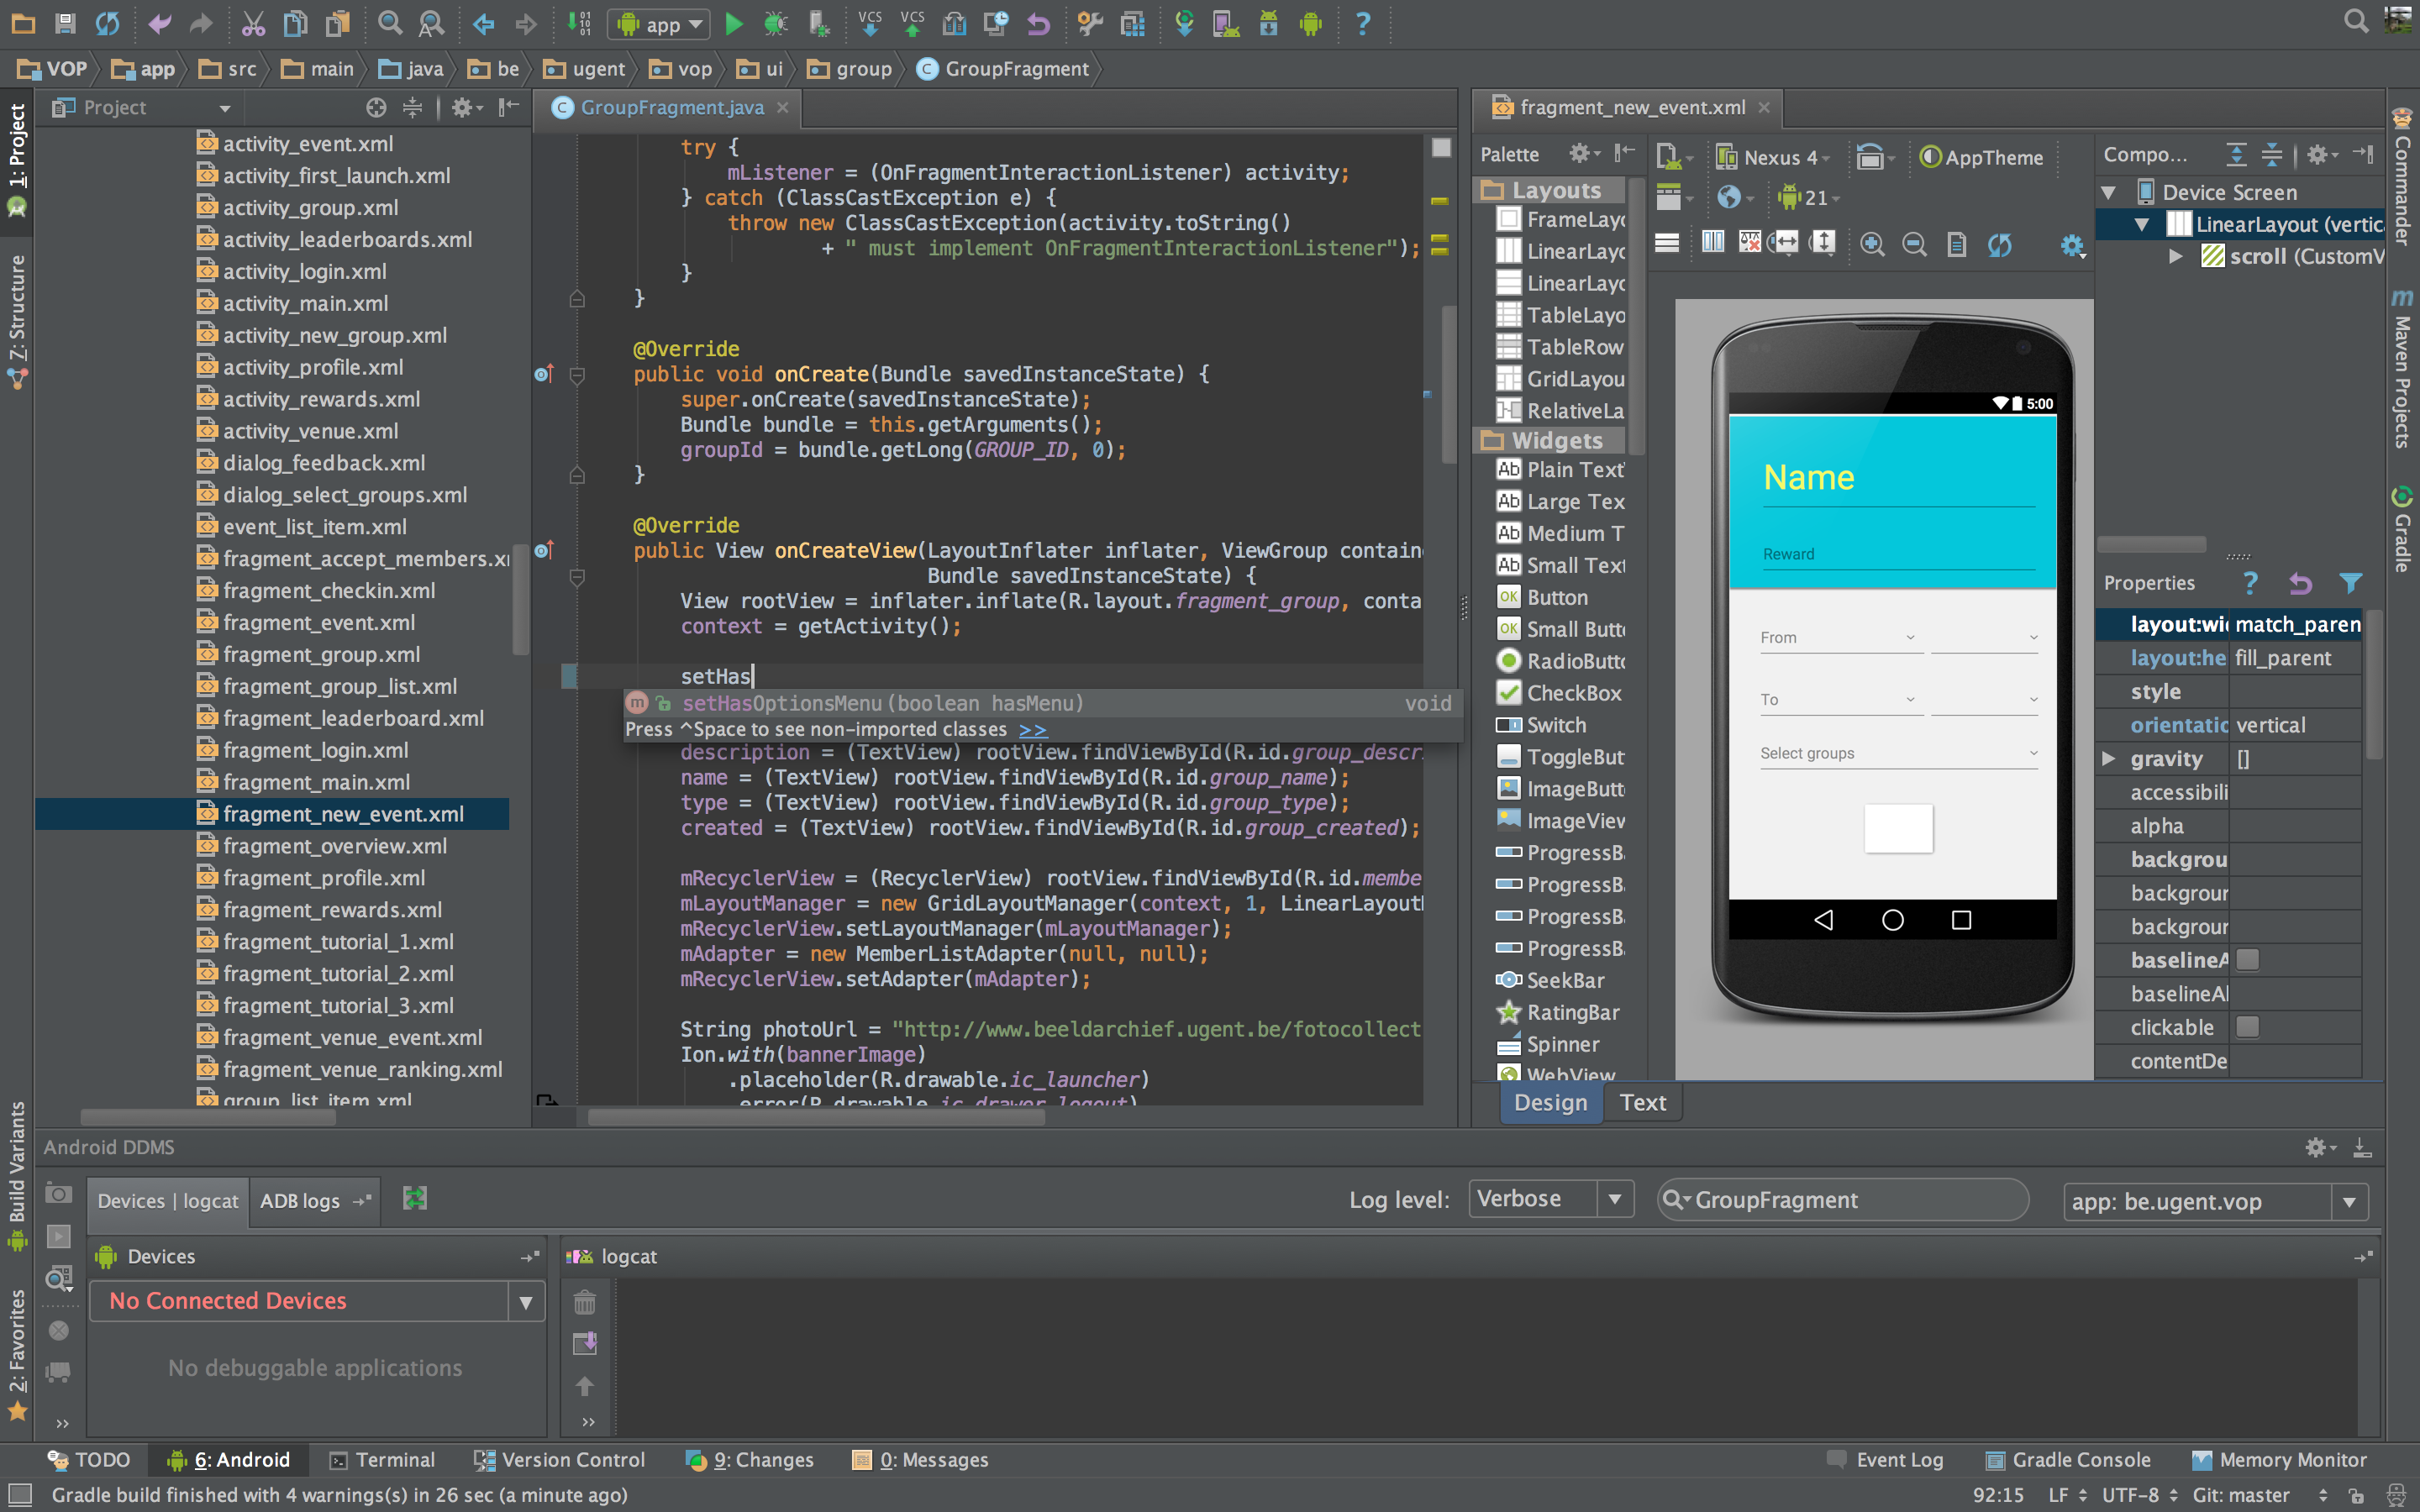
\includegraphics[width=\linewidth]{android_studio}
%	\caption{Een typische workflow in Android Studio}
%	\label{fig:Android Studio Workflow}
%\end{figure}

\subsection{Webinterface}
\label{Webinterface}
\subsubsection{Doel}
Voor een aantal taken is een smartphone niet helemaal geschikt. Zulke taken zijn o.a. het beheren van groepen en het aanmaken van officiele evenementen.
Deze taken gebeuren met bepaalde regelmaat en zijn gemakkelijker op een groter scherm uit te voeren. Specifieke gebruikers, zoals uitbaters van locaties die een promotie willen opzetten als online marketing strategie, zullen deze taken willen uitvoeren via een overzichtelijke webinterface. Daarom is Triump uitgebreid met een webinterface die bereikbaar is via de publieke website van Triump.
Deze site zal tevens dienst doen als infopunt voor huidige en toekomstige gebruikers. Op de site staat informatie over het doel van Triump, en wordt er een link voorzien zodat toekomstige gebruikers de applicatie kunnen downloaden.

Op de website kunnen gebruikers net als in de Android-applicatie inloggen met Foursquare. Het is de bedoeling dat het registreren van een Foursquare-locatie steeds via de website gebeurd, net als het aanmaken van promoties door een eigenaar van een registreerde locatie. Het opleggen van registratie van een locatie door de eigenaar ervan moet ervoor zorgen dat er geen valse promoties worden opgezet. Zonder registratie zou immers iemand een promotie kunnen aanmaken voor een bepaalde locatie zonder dat deze ook daadwerkelijk wordt gegeven.

\subsubsection{Django-framework}
Bij het maken van een website zijn er verschillende keuzes.
Eerst en vooral is er de keuze of er gebruik wordt gemaakt van een bestaand framework, zoals Ruby on Rails, ASP.NET en Django, of dat men zelf de nodige functionaliteit implementeert met bijvoorbeeld PHP.
Bestaande frameworks bieden ruim voldoende functionaliteit aan om de Triump website te verwezenlijken. De frameworks zijn bovendien reeds geoptimaliseerd en bevatten functies zoals een standaardmanier om gebruikers veilig in te loggen. 
Daarnaast moet men nog kiezen om ofwel de site bij een hosting-dienst te plaatsen, ofwel zelf de site te hosten op een eigen pc. Gebruik maken van een bestaande hosting-dienst, is het eenvoudigst. Voor een vast bedrag, per maand of jaar, wordt de website geplaatst op de servers van de hosting-dienst. Deze neemt extra moeilijkheden, zoals het instellen en onderhouden van DNS-servers op zich.
Op de site worden gebruikers aangemaakt waarbij bepaalde informatie wordt opgeslaan, zoals hun Foursquare-identiteit, zodat de gebruiker maar 1 keer met Foursquare moet inloggen. Dit gebeurt aan de hand van een DBMS-systeem. \\

Als framework voor de webinterface werd gekozen voor Django, een framework geschreven in Python. Django maakt het mogelijk om op relatief korte tijd toch een dynamische website te bouwen.
Een voordeel van het werken met Django is dat er hosting-diensten bestaan die zich specialiseren in het hosten van Django-projecten. Wij kozen voor zo een dienst, namelijk http://djangoeurope.com.
Bij deze dienst was er de mogelijkheid te kiezen uit verschillende databasemanagment systemen. Er werd gekozen voor PostgreSQL: een open source DBMS waar reeds mee gewerkt werd tijdens het vak "Databanken".
Dez communicatie verloopt via Javascript en dient om bijvoorbeeld het organiseren van een evenement mogelijk te maken.Google biedt namelijk een API aan die het mogelijk maakt om Google Endpoints via Javascript aan te spreken. Zo wordt gemakkelijk een van de functies uit de backend opgeroepen en kan het resultaat, dat in JSON wordt ontvangen, ook vlot worden verwerkt met behulp van Javascript. Deze keuze brengt wel nadelen met zich mee. Aan de basis van deze nadelen ligt het feit dat Javascript op de computer van de gebruiker wordt uitgevoerd, en niet op de server die de website host. Op sommige computers is Javascript namelijk niet is geïnstalleerd. Het 'client-side' uitvoeren van code brengt nog een ander nadeel met zich mee: het vormt namelijk een zwak punt in de verdediging tegen aanvallen van buitenaf. Een alternatief is het gebruiken van een python-module op de webserver die communicatie met Google Endpoints mogelijk maakt. Deze code wordt 'server-side' uitgevoerd.


\chapter{Ontwerp}
Figuur \ref{fig:algemene structuur backend} geeft een abstract overzicht van de verschillende onderdelen van de backend en van de interacties tussen de backend en de frontend. De pijlen aangeduid in figuur \ref{fig:algemene structuur backend} worden in de volgende secties verklaard.

\begin{figure}[H]
	\centering
	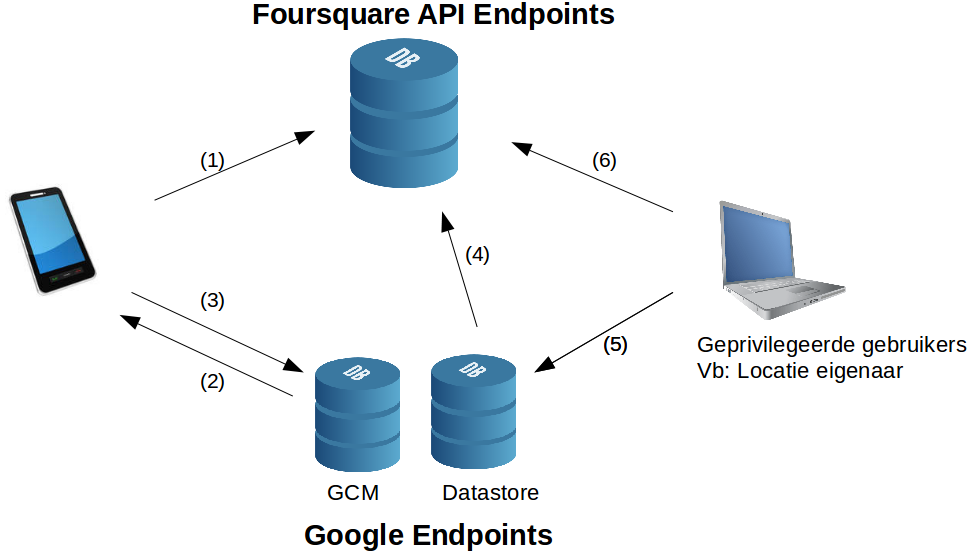
\includegraphics[scale=0.3]{backend_algemene_structuur}
	\caption{Overzicht interactie tussen de frontend en de backend (pijlen worden in onderstaande secties verklaard).}
	\label{fig:algemene structuur backend}
	
\end{figure}
\section{Backend}
\subsection{Database}
Zoals reeds aangegeven word de backend database gehost op een GAE instantie. Deze GAE Datastore is schemaloos wat impliceert dat er geen enkele restrictie met betrekking tot de opbouw van entiteiten wordt opgelegd. M.a.w. maakt GAE Datastore geen gebruik van DDL (Data definition language) om de databank te configureren. Toch is er gekozen voor de database te ontwerpen als een relationele databank aangezien dit toeliet bepaalde operaties zeer efficiënt aan te pakken. Door het ontbreken van de DDL ligt het behoud van de integriteit nu wel volledig bij de ontwikkelaars. 

Figuur \ref{fig:Backend ER} toont een ER diagram van de backend database.  De belangrijkste entiteiten van deze database zijn User, Event, Venue, Group en Checkin. In de volgende paragraaf wordt de structuur van de database besproken. 

Een user entiteit wordt aangemaakt wanneer een gebruiker zich voor het eerst authenticeert bij de backend. Het ID van een gebruiker binnen de Triump database is identiek aan het ID van een gebruiker binnen de Foursquare database. Informatie zoals voornaam, achternaam en e-mailadres van een gebruiker wordt bekomen via een request naar de Foursquare API. In sectie \ref{Foursquare API} komt de werking van de Foursquare API aan bod. Pijl (4) van figuur \ref{fig:algemene structuur backend} geeft de afhankelijkheid tussen Triumps database en de Foursquare database weer.

Venue-entiteiten worden aangemaakt wanneer een gebruiker voor het eerst incheckt op een nieuwe locatie. Opnieuw is de ID van een venue entiteit identiek aan het ID van de entiteit binnen Foursquare. Een datum en tijdstip van de eerste checkin wordt bijgehouden. Deze informatie kan gebruikt worden om statistieken van locaties te genereren. Een locatie of venue heeft een `verified' attribuut indien een gebruiker zich via de webinterface (zie sectie \ref{Webinterface} voor meer informatie over het doel en de werking van de webinterface) verifieert. Een geverifieerde gebruiker (meestal een locatie-eigenaar) in combinatie met een geverifieerde locatie kan een evenement organiseren waaraan elke groep, indien zij voldoen aan de opgelegde participatievoorwaarden, kan deelnemen. Aan de winnaar van het evenement kan dan een promotie toegekend worden.

Zoals reeds aangehaald zijn er enerzijds `officiële' evenementen waarbij promoties verkregen kunnen worden. Anderzijds zijn er ook evenementen die gebruikers voor hun vrienden organiseren. Deze evenementen kunnen aangemaakt worden door elke gebruiker. Aangezien deze gewone evenementen niet automatisch zichtbaar zijn moet de organisator groepen, waartoe hij of zij zelf behoort, uitnodigen. 
Deze twee types evenementen worden beiden opgeslagen in Event-entiteiten. Het `verified' veld geeft aan of een Event entiteit een officieel of gewoon Event is. De attributen minParticipants en maxParticipants hebben enkel een geldige waarde voor evenententen met promoties. De organisator hiervan kan beslissen een verschillende promotie te lanceren afhankelijk van de groepgrootte. De entiteit GroupEvent wordt gebruikt om bij te houden welke groepen er zijn uitgenodigd op een gewoon evenement.


\begin{figure}[H]
	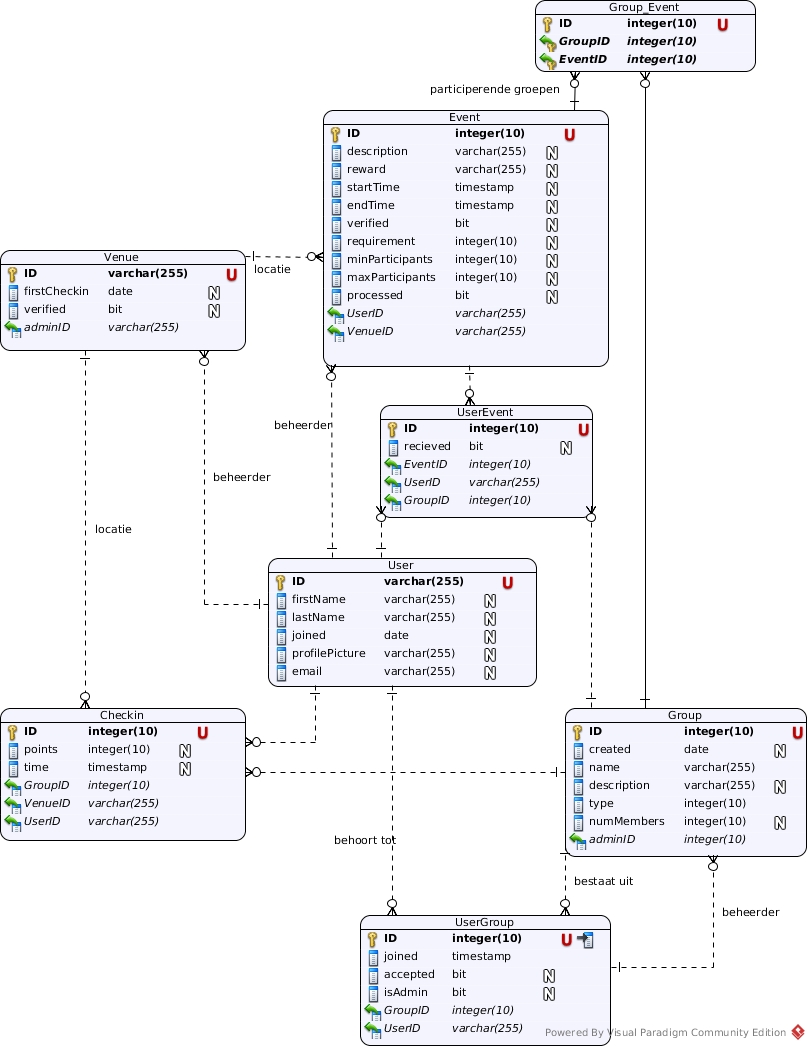
\includegraphics[scale=0.43]{backend_EER}
	\caption{Entity Relation diagram van de backend database}
	\label{fig:Backend ER}
\end{figure}


Een Checkin entiteit wordt aangemaakt iedere keer een gebruiker incheckt op een locatie. Het `points' veld geeft aan hoeveel punten een checkin waard is. In de huidige implementatie geldt er dat elke checkin 1 punt waard is. Het is echter mogelijk de app uit te breiden en te voorzien dat bepaalde combinaties van inchecken meer punten opleveren. De attributen tijdstip en groep worden bijgehouden om te bepalen welke groep een event heeft gewonnen (doordat de groep het meest heeft ingechecked) en om de ranglijsten op te stellen. (Meer informatie over deze berekeningen volgt in sectie \ref{backend API}: Backend API.)


Elke gebruiker van Triump is in staat zijn eigen groepen aan te maken. De maker van een groep is ook de administrator ervan. Opnieuw kan het `type' attribuut gebruikt worden om statistieken te generen van de beste studentvereniging of meest actieve vriendengroep. `numMembers' is afgeleide data aangezien de waarde kan berekend worden uit het aantal entiteiten in de UserGroup tabel. Toch wordt `numMembers' bijgehouden in Group-entiteiten aangezien dit een waarde is die vaak gebruikt wordt. Voordelen hiervan zijn een verbetering van de performantie en een vermindering van het aantal leesoperaties. Een nadeel is de mogelijkheid tot het optreden van anomalieën (vb: indien `numMembers' niet overeenstemt met het aantal entiteiten in UserGroup voor een bepaalde groep).

UserGroup-entiteiten koppelen een gebruiker met een groep. Een entiteit wordt aangemaakt wanneer een gebruiker een aanvraag doet om tot een groep te behoren. Het `accepted' attribuut wordt bij de aanmaak op 0 geplaatst tot de administrator toestemming geeft aan de gebruiker om lid te worden van de groep. Indien de administrator het lidschapverzoek weigert, wordt de entiteit verwijderd.

Tot slot wordt in UserEvent-entiteiten bijgehouden welke gebruikers een promotie/evenement gewonnen hebben en bijgevolg van de promotie gebruik mogen maken. Het `received' attribuut geeft aan indien een gebruiker zijn prijs reeds heeft gebruikt. Ook deze data kan interessant zijn voor de officïele gebruikers om bij te houden hoeveel mensen gebruik maken van de georganiseerde evenementen/promoties.

Het ontwerp van de backend database focust enerzijds op functionaliteit (alle functies die Triump wil aanbieden moeten namelijk mogelijk zijn met de backend) en anderzijds op het bijhouden van informatie voor statistieken. Indien Triump gebruikt zal worden als online marketing tool, is het belangrijk om statistieken te genereren over het gebruik van de toepassing om zo locatie-eigenaars aan te kunnen geven hoe ze Triump het best gebruiken. Bovendien zijn statistieken ook voor gebruikers interessant.

Figuur \ref{fig:Backend ER 2} toont het overige deel van de backend database. Wanneer een gebruiker zich voor het eerst authenticeert met de backend wordt er een SessionToken gekoppeld met de gebruiker. Deze token wordt meegegeven als parameter met iedere API call om de een gebruiker te authenticeren. De GCM tabel van de backend database houdt voor iedere gebruiker een gcmId bij. Deze ID wordt gebruikt voor de Google Cloud Messaging dienst.

\begin{figure}[H]
	\centering
	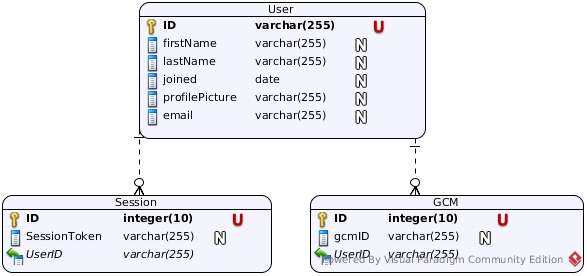
\includegraphics[scale=0.45]{backend_EER_deel2}
	\caption{Entity Relation diagram van het administratieve deel van de backend database}
	\label{fig:Backend ER 2}
\end{figure}
\subsection{Google Cloud Messaging}
GCM wordt in Triump gebruikt als basis van het notificatie systeem. In de huidige implementatie ontvangt een gebruiker een notificatie indien hij/zij een event heeft gewonnen of indien er om feedback wordt gevraagd. 
Pijl (2) van figuur \ref{fig:algemene structuur backend} geeft aan dat er via GCM, vanop de backend servers, berichten worden gepusht naar de gebruikers.

\subsection{Cron jobs}
In het geval van de backend van Triump is het noodzakelijk om beloningen (rewards) na het aflopen van evenementen voor gebruikers te laten genereren. Hiervoor wordt gebruik gemaakt van een cron job, die geconfigureerd wordt in een Java servlet. 

\subsection{Backend API}
\label{backend API}
De backend API bestaat uit een reeks methodes die kunnen opgeroepen worden vanop het mobiele toestel of vanop de webinterface. Dit is weergegeven met pijlen (3) en (5) op figuur \ref{fig:algemene structuur backend}. Een groot deel van de methodes hebben als doel het ophalen van gegevens uit de database, deze gegevens te mappen op een klasse om vervolgens een object terug te geven als resultaat. Deze objecten worden vervolgens gemanipuleerd in de Android toepassing of de webinterface.

Een tweede soort API calls wordt gebruikt om entiteiten van de tabellen Group, Event, UserGroup en UserEvent aan te maken of te wijzigen. Een van deze methoden is generateRewards(). De methode generateRewards() wordt vanuit een Cron Job (zie sectie \ref{sec: GCE} Cron jobs) ieder kwartier opgeroepen. Prinicpieel werkt de functie als volgt:
\begin{enumerate}
	\item Controleer of er het afgelopen kwartier een event is beëindigd.
	\item Bereken voor elk beëndigd event welke groepen gewonnen zijn a.d.h.v. de tijdstippen van de Checkin entiteiten. Hierbij wordt er rekening gehouden met participatievoorwaarden zoals het minimaal en maximaal aantal leden van een groep.
	\item De leden van een winnende groep worden geplaast in de UserEvent tabel.
	\item Via het notificatiesysteem (zie sectie \ref{sec: GCE} Google Cloud Messaging) worden de winnende gebruikers verwittigd.
\end{enumerate}
Voor elke functie in de backend is een algoritme uitgewerkt waarbij steeds rekening gehouden wordt met efficiëntie (wegens het beperkt aantal atomaire operaties aangeboden door GCE, zie \ref{sec: GCE})
Tot slot bevat de backend API nog methodes die gebruikers registeren, gebruikers authenticeren en communiceren met de GCM diensten. 

\subsection{Foursquare API}
Het mobiele toestel zal rechtstreeks requests sturen naar de Foursquare API om bijvoorbeeld een lijst te krijgen van dichtbijzijnde locaties of om informatie van een locatie op te vragen. Het gebruik van de API wordt getoond in figuur \ref{fig:algemene structuur backend} via pijl (1).


\section{Frontend}
\subsection{Android applicatie}

\subsubsection{Ontwerpkeuzes}
Tijdens de ontwikkeling van Triump is er voor gekozen om te werken met de nieuwste technologieën voor Android. Dat houdt in dat Triump ontwikkelt is met als doel volledig compatibel te zijn met de laatste versie van Android: 5.1 Lollipop. Triump is daarnaast wel nog steeds compatibel met alle Android versies vanaf 4.1 Jelly Bean. Hierdoor bereikt de applicatie 87,5\% van alle Android toestellen \cite{market_share}. 
Android development gebeurd in Java, maar er zijn enkele Android-specifieke ontwerppatronen waarvan er gebruik gemaakt wordt. Onder andere voor het asynchroon laden van informatie, het opslaan van data en het opbouwen van efficiënte UI lijsten zijn er speciale ontwerppatronen in Android. Deze zullen in de volgende secties verder uitgelegd worden.

\subsubsection{Material Design}
Triump is ontwikkeld voor Android Lollipop. Dit houdt in dat er gebruik gemaakt wordt van de Material Design Guidelines \cite{Material_Design}. Door de Material Design Guidelines te volgen is het makkelijker om een consistent look-and-feel te verkrijgen in de app die volledig in lijn ligt met de rest van het Android ecosysteem.
Om de correcte implementatie van Material Design te garanderen, is er gebruik gemaakt van enkele externe bibliotheken. Deze bibliotheken bieden extra functionaliteit ten opzichte van de standaard Android API waardoor het makkelijker is het correcte design te verkrijgen. Deze bibliotheken zijn steeds backwards compatible met eerdere versies van Android. Hierdoor wordt er een uniforme look verkregen op alle versies die de app ondersteunt.
De gebruikt bibliotheken om Material Design te implementeren zijn:
\begin{description}
	\item[Material Design Library \cite{navasmdc}] Een bibliotheek die verschillende UI componenten bevat die voldoen aan de Material Design Guidelines zoals de Flat Buttons, Progress Bar Indicators en Switches.
	\item[FloatingActionButton \cite{floatingactionbutton}] Een bibliotheek die de Floating Action Button van de Material Design Specification implementeert en toelaat om die toe te voegen aan een RecyclerView (zie verder).
	\item[MaterialEditText \cite{materialedittext}] Een bibliotheek die een consistent implementatie biedt voor tekstvelden in formulieren. De bibliotheek voorziet verschillende functies voor de tekstvelden zoals maximum lengte, hints, iconen en aangepaste kleuren.
\end{description}

\subsubsection{RecyclerView}
Sinds Android 5.0 is er een nieuwe manier geïntroduceerd om lijsten weer te geven in de UI van de applicatie. Onze applicatie maakt veelvuldig gebruik van lijsten (groepen, locaties, evenementen,...) en bijgevolg wordt gestreefd van de laatste standaard hieromtrent gebruik te maken. Deze nieuwe widget (zo heten de UI componenten in Android) is de RecyclerView. De RecyclerView vervangt de oudere ListView widget.
De ListView en RecyclerView geven beiden een lijst weer van data. Beide widgets worden aangestuurd door een zogenaamde DataAdapter. Die Adapter is een speciale klasse die de widgets oproepen om de rijen van de lijsten te vullen met data. Daarvoor moet de Adapter bepaalde methoden implementeren die dan door de ListView / RecyclerView opgeroepen worden. Bij zowel ListView als RecyclerView is 1 van die methodes verantwoordelijk voor het vullen van de View van 1 rij met de correcte data.
Voor elke rij in de lijst is de layout vastgelegd in een XML bestand. Aan de hand van dit XML bestand wordt dan voor elke rij een View object aangemaakt dat de correcte layout bevat voor die rij. Op dat moment is het View object voor die rij nog niet gevuld met de correcte data. Daarvoor wordt bij de Adapter een methode opgeroepen om die View te vullen met de correcte data.
Het is in deze stap dat RecyclerView en ListView fundamenteel verschillen. In het geval van een ListView zal de Adapter voor elke rij verschillende findViewById(int id) operaties moeten doen om de correcte sub-View van de View van de rij te verkrijgen. Dat is nodig omdat de Adapter een referentie moet verkrijgen naar bijvoorbeeld een label View binnen de View van de rij. Deze findViewById(int id) operaties zijn echter zeer cpu-intensief. Hierdoor is scrollen in traditionele ListViews niet zo vloeiend.
RecyclerView maakt het grootste deel van de findViewById(int id) operaties overbodig door standaard gebruik te maken het ViewHolder patroon.
Concreet leidt het nastreven van de laatste Android ontwerppatronen, zoals de RecyclerView, tot een efficiëntere applicatie.

\subsubsection{Loaders}
In Android gebeurt het tekenen en het interageren met de UI, net zoals bij de meeste andere GUI toolkits op de main thread. Dit betekent dat het inladen van data over het netwerk of van de lokale opslag in een aparte thread moeten plaatsvinden. Is dit niet het geval, dan zal de volledige UI blokkeren want aanleiding kan geven tot een slechtere gebruikerservaring.
Om deze redenen bevat Android het concept van Loaders. De bedoeling van Loaders is om data op een asynchrone manier in te laden (dus op een aparte thread) en de resultaten via een callback terug te sturen naar de main UI thread teneinde ze op het scherm weer te geven. 
\newline\newline

De Material Design richtlijnen, Recycler View en Loaders zijn slechts enkele van de methodes die gevolgd werden bij het ontwikkelen van de Android applicatie. Gedurende het volledige ontwerpproces werd op deze manier gestreeft naar een zo efficiënt mogelijke applicatie, ontwikkelt volgens de meest recente standaarden. \cite{successapp}
\subsection{Webinterface}
\begin{figure}[H]
	\centering
	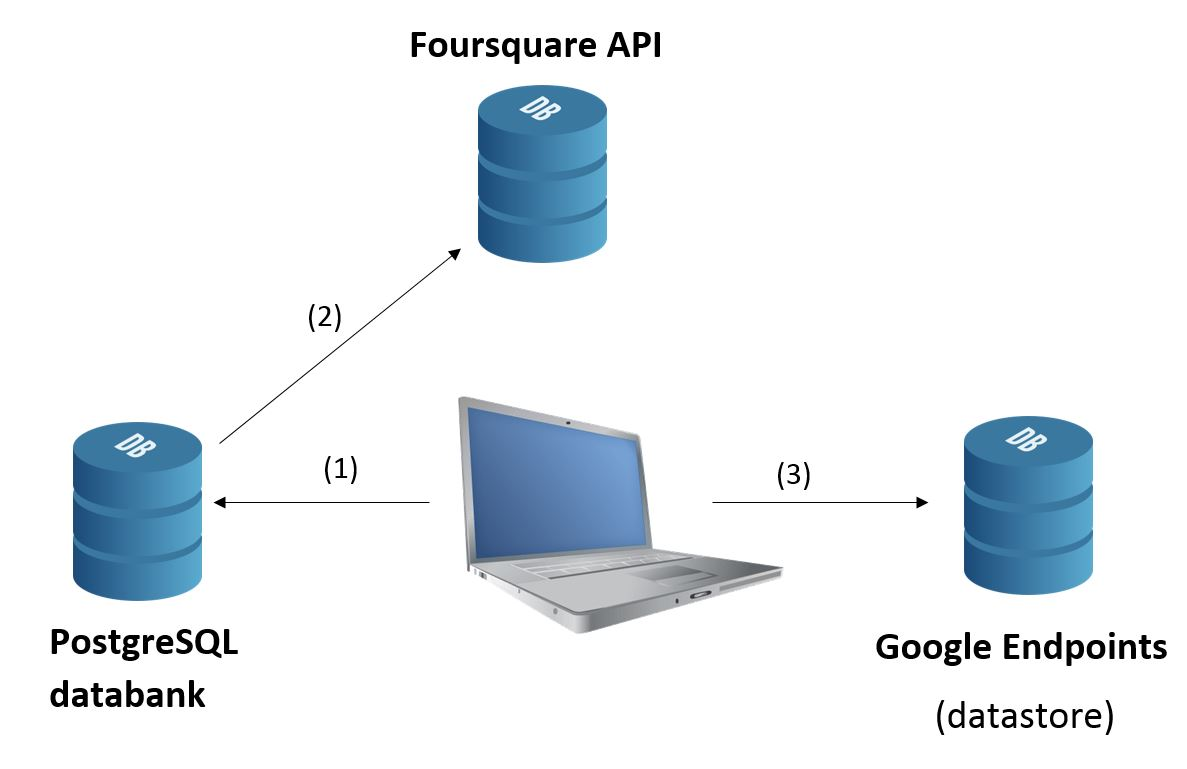
\includegraphics[scale=0.3]{webinterface_structuur}
	\caption{Werking en opbouw webinterface. Zowel de backend datastore als de Foursquare API, via een postgreSQL databank, bieden data aan voor de webinterface. }
	\label{fig:Webinterface}
\end{figure}
De opbouw en werkwijze van de webinterface wordt weergegeven in \ref{fig:Webinterface}. Men kan zien dat de server, die de website host, geconnecteerd is met een PostgreSQL databank (weergegeven met pijl (1)). Deze maakt het mogelijk om gebruikers te laten inloggen met een eigen account, waarbij men ook extra data kan opslaan. Er werd reeds aangehaald dat gebruikers ook hier met Foursquare dienen in te loggen, dit gebeurt na het registreren. Zoals te zien op de figuur gebeurt alle communicatie met de Foursquare API vanop de webserver (weergegeven met pijl (2)), niet door de computer van de gebruiker. Deze communicatie omvat het ophalen van locatie- en gebruikergegevens uit de databank van Foursquare.
Daarnaast kan men op de figuur zien dat er vanop de computer van de gebruiker wordt gecommuniceerd met de backend (GAE) van Triump (weergegeven met pijl (3)). Deze verbinding maakt het mogelijk om vanop de webinterface nieuwe events aan te maken en groepen te beheren.



\chapter{Resultaten en functionaliteit}
In deze sectie worden enkel de resultaten met betrekking tot de frontend besproken, vermits de backend reeds uitvoerig is geanalyseerd in het onderdeel `Ontwerp'.
\section{Android applicatie}
De Android applicatie werd geprogrammeerd in 10 weken en is bijgevolg slechts een prototype. Desalniettemin bevat de applicatie reeds alle functionaliteit en is ook op vlak van UI een intuïtieve interface uitgedacht.
De applicatie is uitgebouwd rond 1 centraal scherm. Hieruit kan rechtstreeks genavigeerd worden naar het Overview-, Checkin- en Groupscherm (Fig. \ref{fig:screenshot_overview}). Deze 3 schermen bevatten alle vereiste functies die een gebruiker normaal gezien nodig heeft (inchecken, controleren van de evenementen/promoties en groepsactiviteit). Andere functionaliteit (innen van promoties, bekijken van alle groepen en evenementen, instellingen,...) is beschikbaar via het `navigation drawer' mechanisme. Dit is een paneel met navigeermogelijkheden dat zichtbaar wordt door het vegen naar rechts. De layout van de Android applicatie is gekozen na analyse van verschillende Android applicaties en huidige ontwikkelstandaarden voor Android toepassingen. Daarnaast wordt een uniforme interface voorzien, conform met de Material Design standaarden. In volgende onderdelen wordt van de verschillende schermen de functionaliteit besproken. Screenshots hiervan worden bijgevoegd onder elke sectie.
\subsubsection{Login en tutorial} %Lars
Bij het eerste keer opstarten van de Android applicatie wordt een tutorialsequentie (Fig. \ref{fig:screenshot_login}) opgestart. Hierin wordt de doelstelling van de applicatie uitgelegd en wat de verschillende mogelijkheden zijn. Indien na feedback van gebruikers blijkt dat deze schermen niet voldoende intuïtief zijn, kan deze tutorial uitgebreid worden met enkele schermen waarbij de eigelijke applicatie getoond wordt en ingezoomd worden op de specifieke functionaliteit en navigatie doorheen de toepassing. 
Na de tutorialsequentie wordt de gebruiker gevraagd om in te loggen (Fig. \ref{fig:screenshot_profile}). Vermits het doel van deze applicatie het uitbreiden van de Foursquare/Swarm functionaliteit is, wordt de gebruiker gevraagd om in te loggen met zijn/haar Foursquare/Swarm account. Het inloggen vereist het installeren van de Foursquare/Swarm applicatie. Op deze manier kan Triump steunen op de reeds bestaande gebruikers van Foursquare/Swarm. Bovendien kan hierdoor het volledig login/registreerproces uitbesteed worden en kan een bestaande API gebruikt worden.
Na de eerste keer inloggen wordt de gebruiker `geïnitialiseerd' op de backend van Triump.
\begin{figure}[ht]
\begin{minipage}[b]{0.18\linewidth}
	\centering
	
\includegraphics[width=\textwidth]{shot_tutorial}
	\caption{Tutorial}
	\label{fig:screenshot_login}
\end{minipage}
\hspace{2.4cm}
\begin{minipage}[b]{0.18\linewidth}
\centering
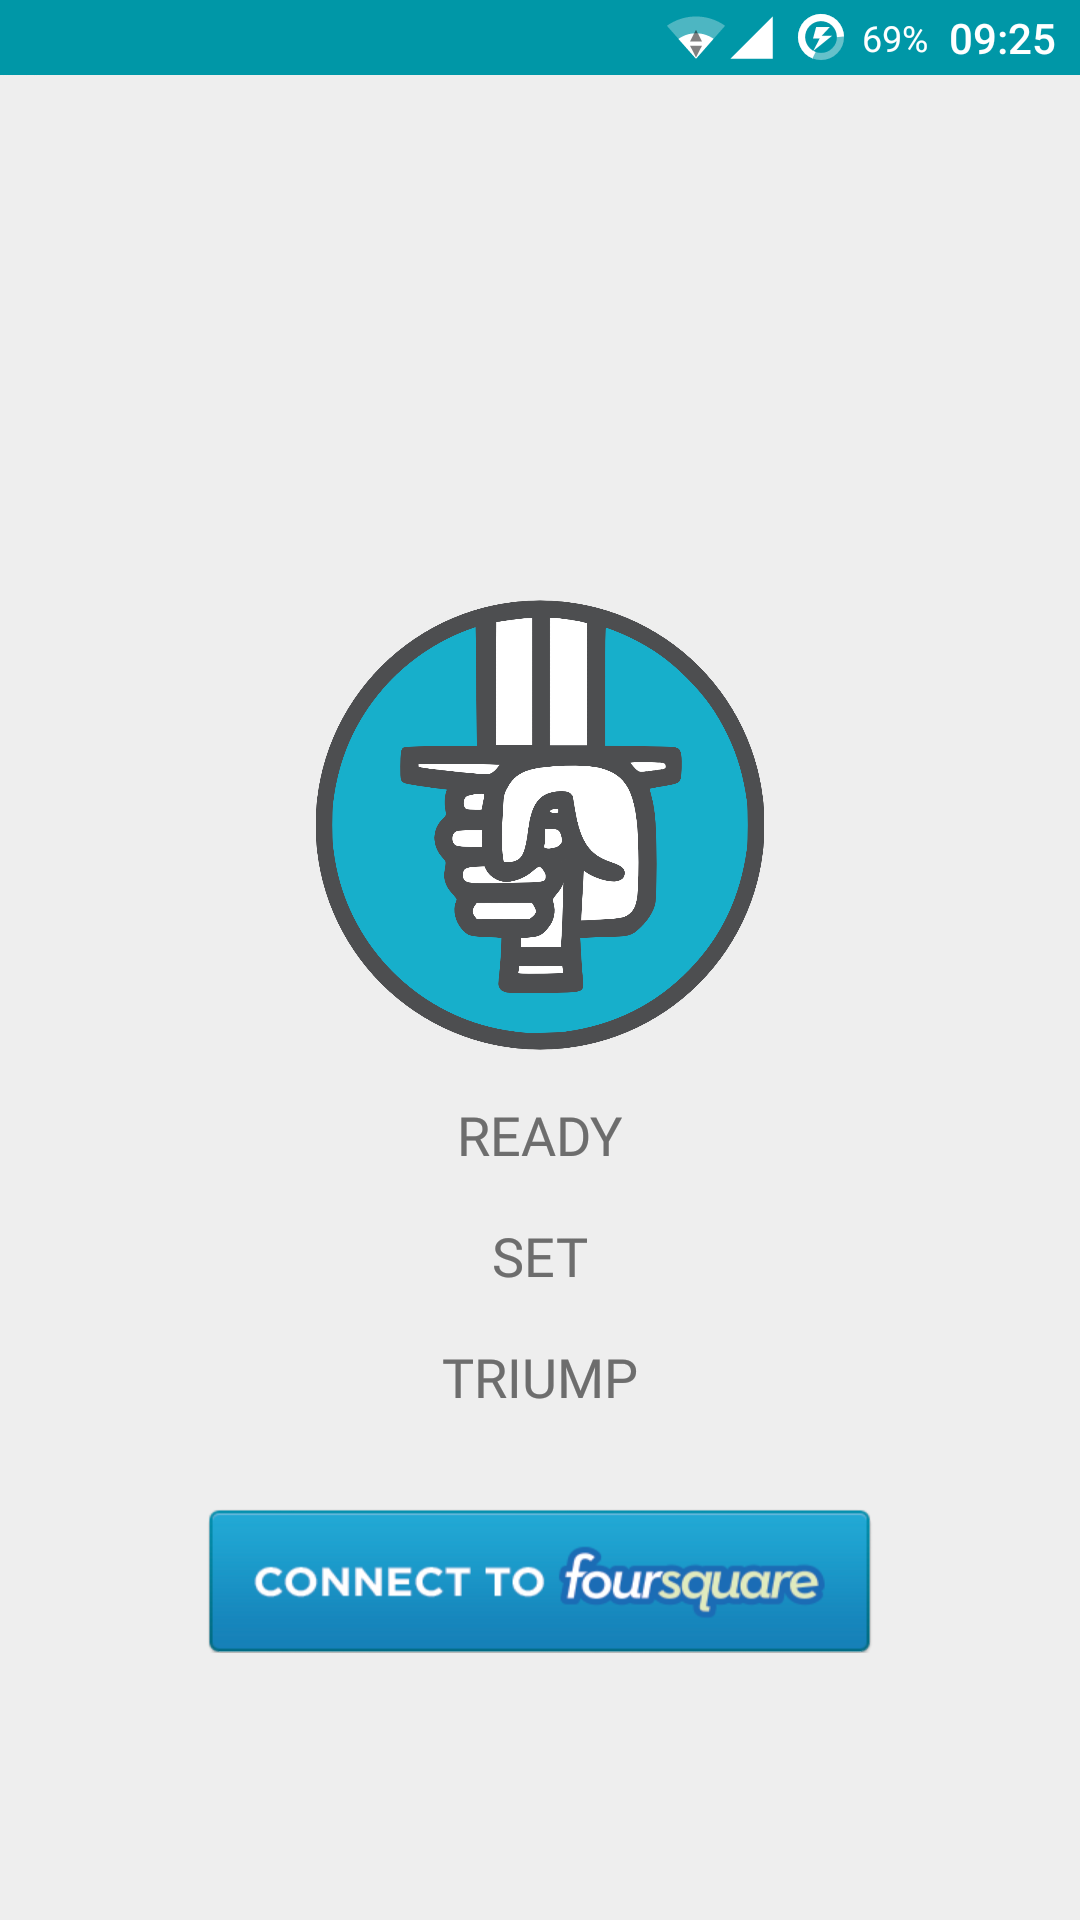
\includegraphics[width=\textwidth]{shot_login}
\caption{Login}
\label{fig:screenshot_profile}
\end{minipage}
\hspace{2.4cm}
\begin{minipage}[b]{0.18\linewidth}
\centering
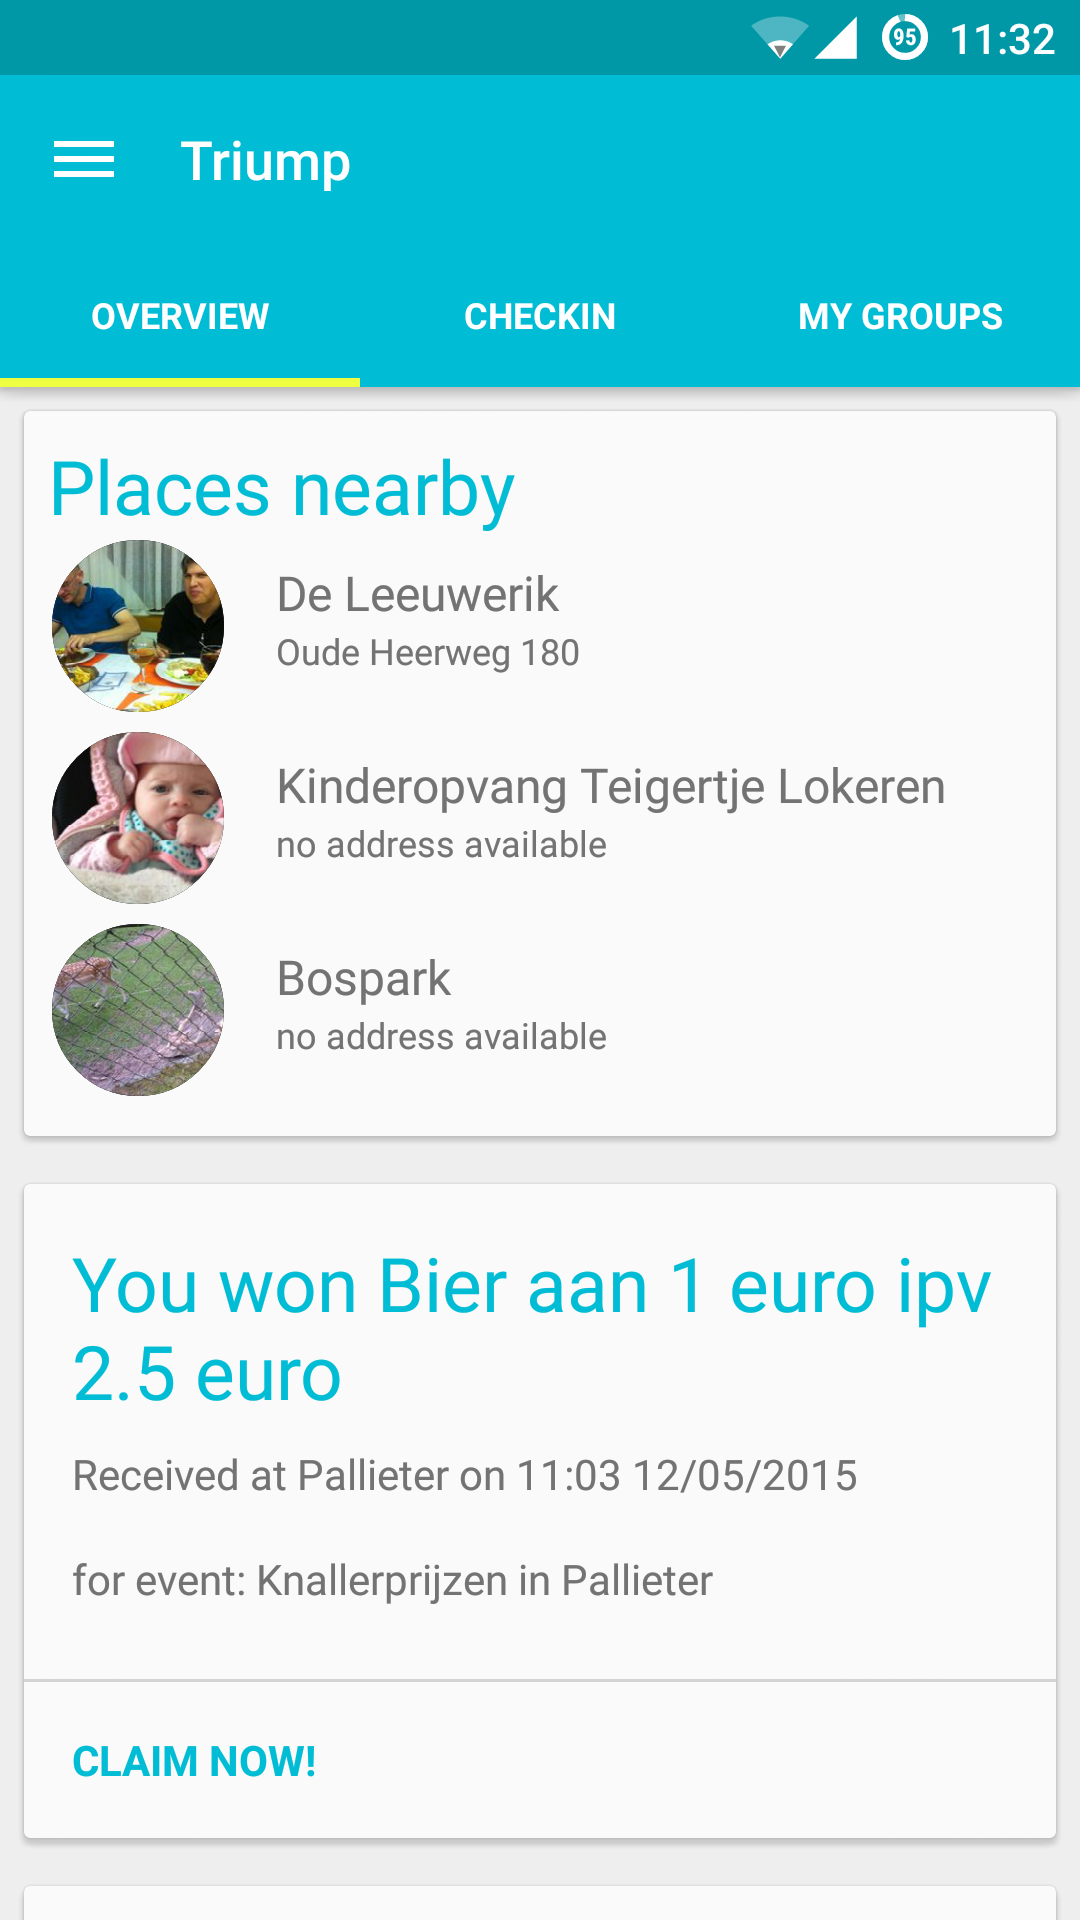
\includegraphics[width=\textwidth]{shot_overview1}
\caption{Overzicht}
\label{fig:screenshot_overview}
\end{minipage}
\end{figure}
\clearpage
\subsubsection{Overview en notificaties} %Lars
Om gebruikers op de hoogte te houden van recente activiteit van hun groepen, events die aan de gang zijn, promoties, checkins,... worden in de Android applicatie 2 mechanismen voorzien. 
Enerzijds is er het Overviewscherm (Fig. \ref{fig:screenshot_overview2}), het eerste scherm dat de gebruiker ziet in de applicatie, anderzijds zijn er de notificaties.
Het Overviewscherm wordt dynamisch gegenereerd op basis van de activiteit van de gebruikers. Hiervoor wordt met `CardViews' in een RecyclerView gewerkt, waardoor ze efficiënt kunnen voorgesteld worden in een lijst en interactief zijn. Het Overviewscherm toont de checkins van groepsleden , evenementen in de buurt en gewonnen promoties. Op deze manier kan de gebruiker vanuit het Overviewscherm navigeren naar andere onderdelen binnen de applicatie (evenementen, ranglijsten, groepen, checkin...).
Naast het Overviewscherm, wordt de gebruiker van updates voorzien via notificaties. Deze notificaties hebben betrekking op evenementen en promoties (voor checkins worden geen notificaties verstuurd om de gebruiker niet te belasten met overbodige notificaties). Bovendien heeft de gebruiker de mogelijkheid om notificaties uit te schakelen via de instellingen. Notificaties kunnen ook occasioneel gebruikt worden om aan de gebruiker feedback te vragen via het Feedbackscherm. Voornamelijk in de ontwikkel- en testfase is dit van belang.
Kortom, het Overviewscherm en de notificaties zijn een interactieve manier om de gebruikers aan te zetten tot het gebruiken van de applicatie.

\subsubsection{Checkin}%Siebe
Om integratie met de diensten van Swarm te voorzien wordt een gelijkaardige interface om in te checken gebruikt. Een Location service controleert de locatie van de gebruiker en toont op de kaart de naburige Foursquare locaties (Fig. \ref{fig:screenshot_checkin}). De gebruiker kan vervolgens uit een dynamisch schaalbare lijst de locatie kiezen waar men wil inchecken. Indien de gebruiker niet geïnteresseerd is om in te inchecken, maar enkel de ranglijsten of evenementen wil controleren op een bepaalde locatie, kan dit door de locatie in te typen in het zoekveld. Bij het selecteren van een locatie (via de kaart of via de zoekfunctionaliteit) krijgt de gebruiker een overzicht van de locatie (Fig. \ref{fig:screenshot_venue}). Dit overzicht bestaat steeds uit 2 onderdelen, namelijk de ranglijsten en de evenementen. De gebruiker kan van ranglijst wisselen (voor verschillende groottes of types van groepen). Daarnaast kan de gebruiker, indien hij voldoende dicht is bij de locatie , inchecken voor zijn groepen. Indien de gebruiker een locatie via de zoekfunctionaliteit heeft opgezocht, maar te zich hiervan te ver bevindt, is inchecken niet mogelijk. Men kan wel steeds  de verschillende evenementen te bekijken in het Event onderdeel.
\begin{figure}[ht]
\begin{minipage}[b]{0.25\linewidth}
\centering
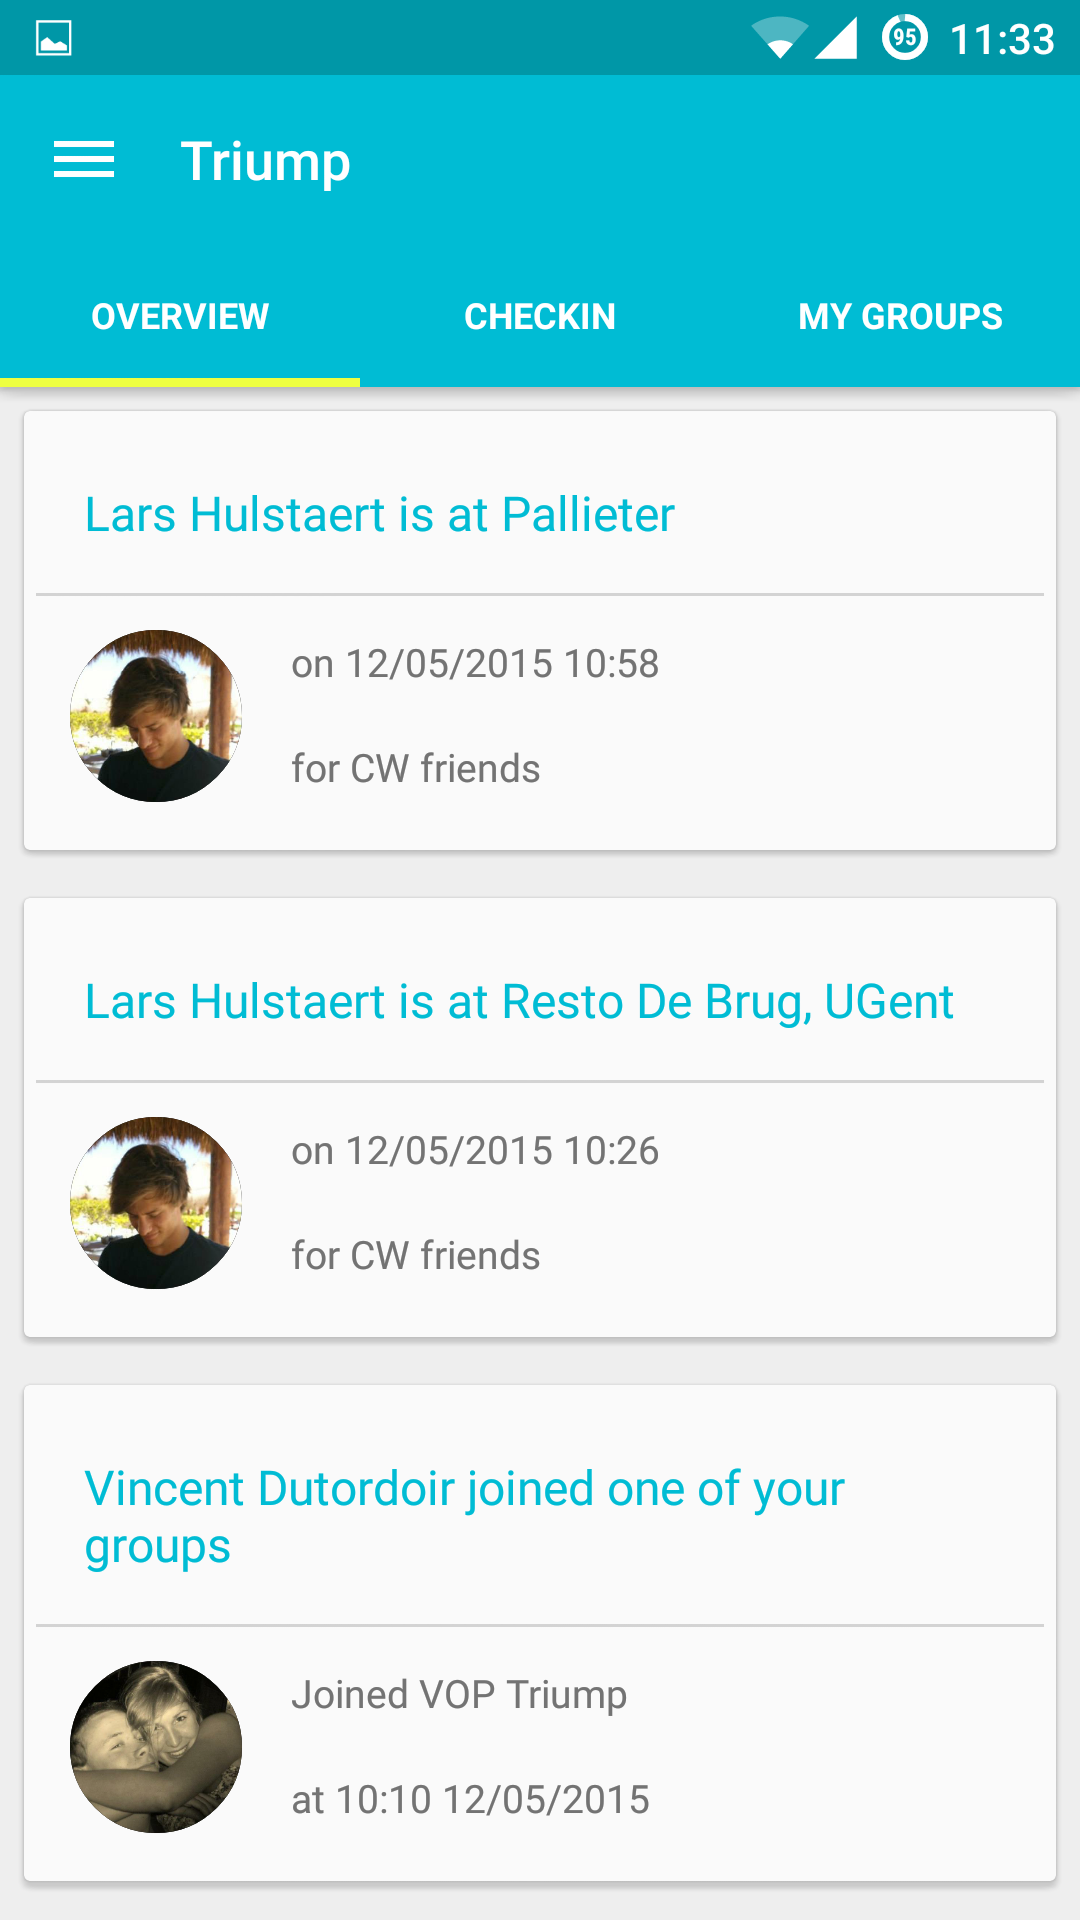
\includegraphics[width=\textwidth]{shot_overview2}
\caption{Overzicht}
\label{fig:screenshot_overview2}
\end{minipage}
\hspace{1.5cm}
\begin{minipage}[b]{0.25\linewidth}
\centering
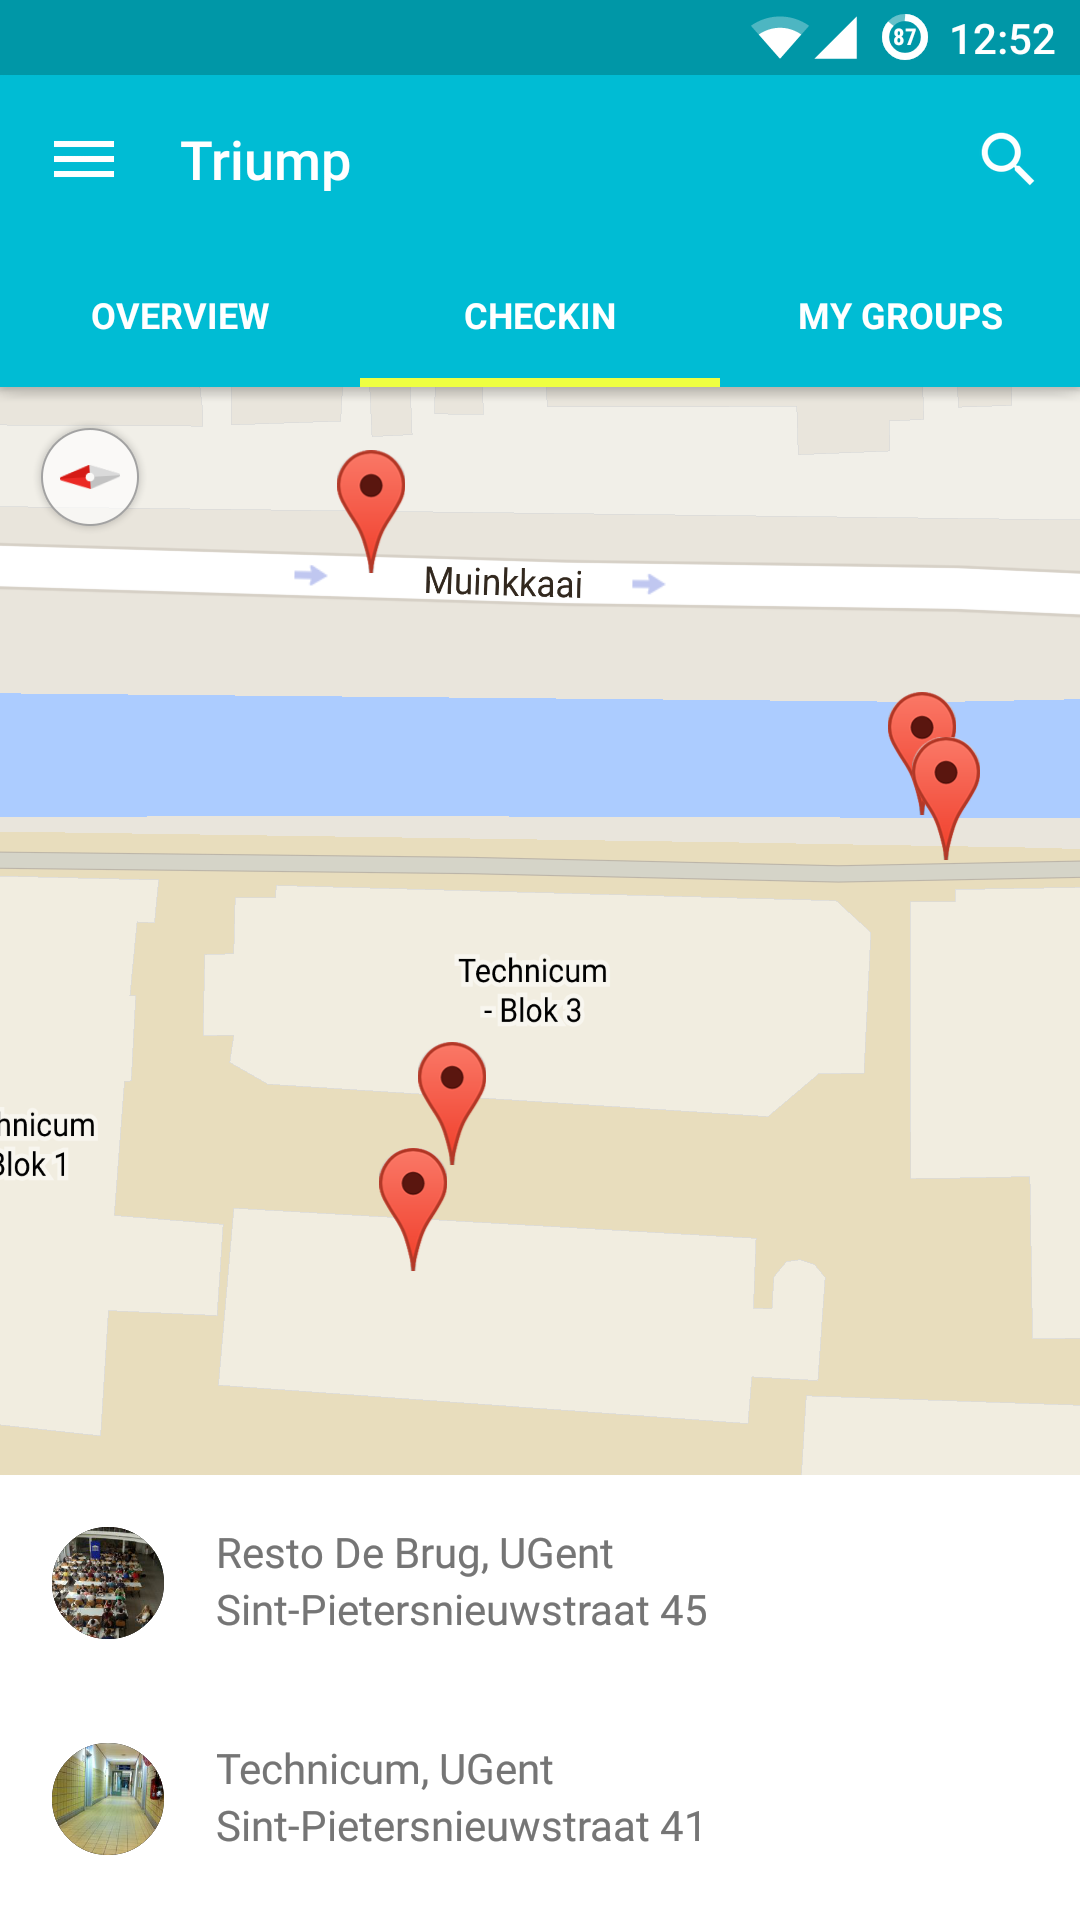
\includegraphics[width=\textwidth]{shot_checkin}
\caption{Checkin}
\label{fig:screenshot_checkin}
\end{minipage}
\hspace{1.5cm}
\begin{minipage}[b]{0.25\linewidth}
\centering
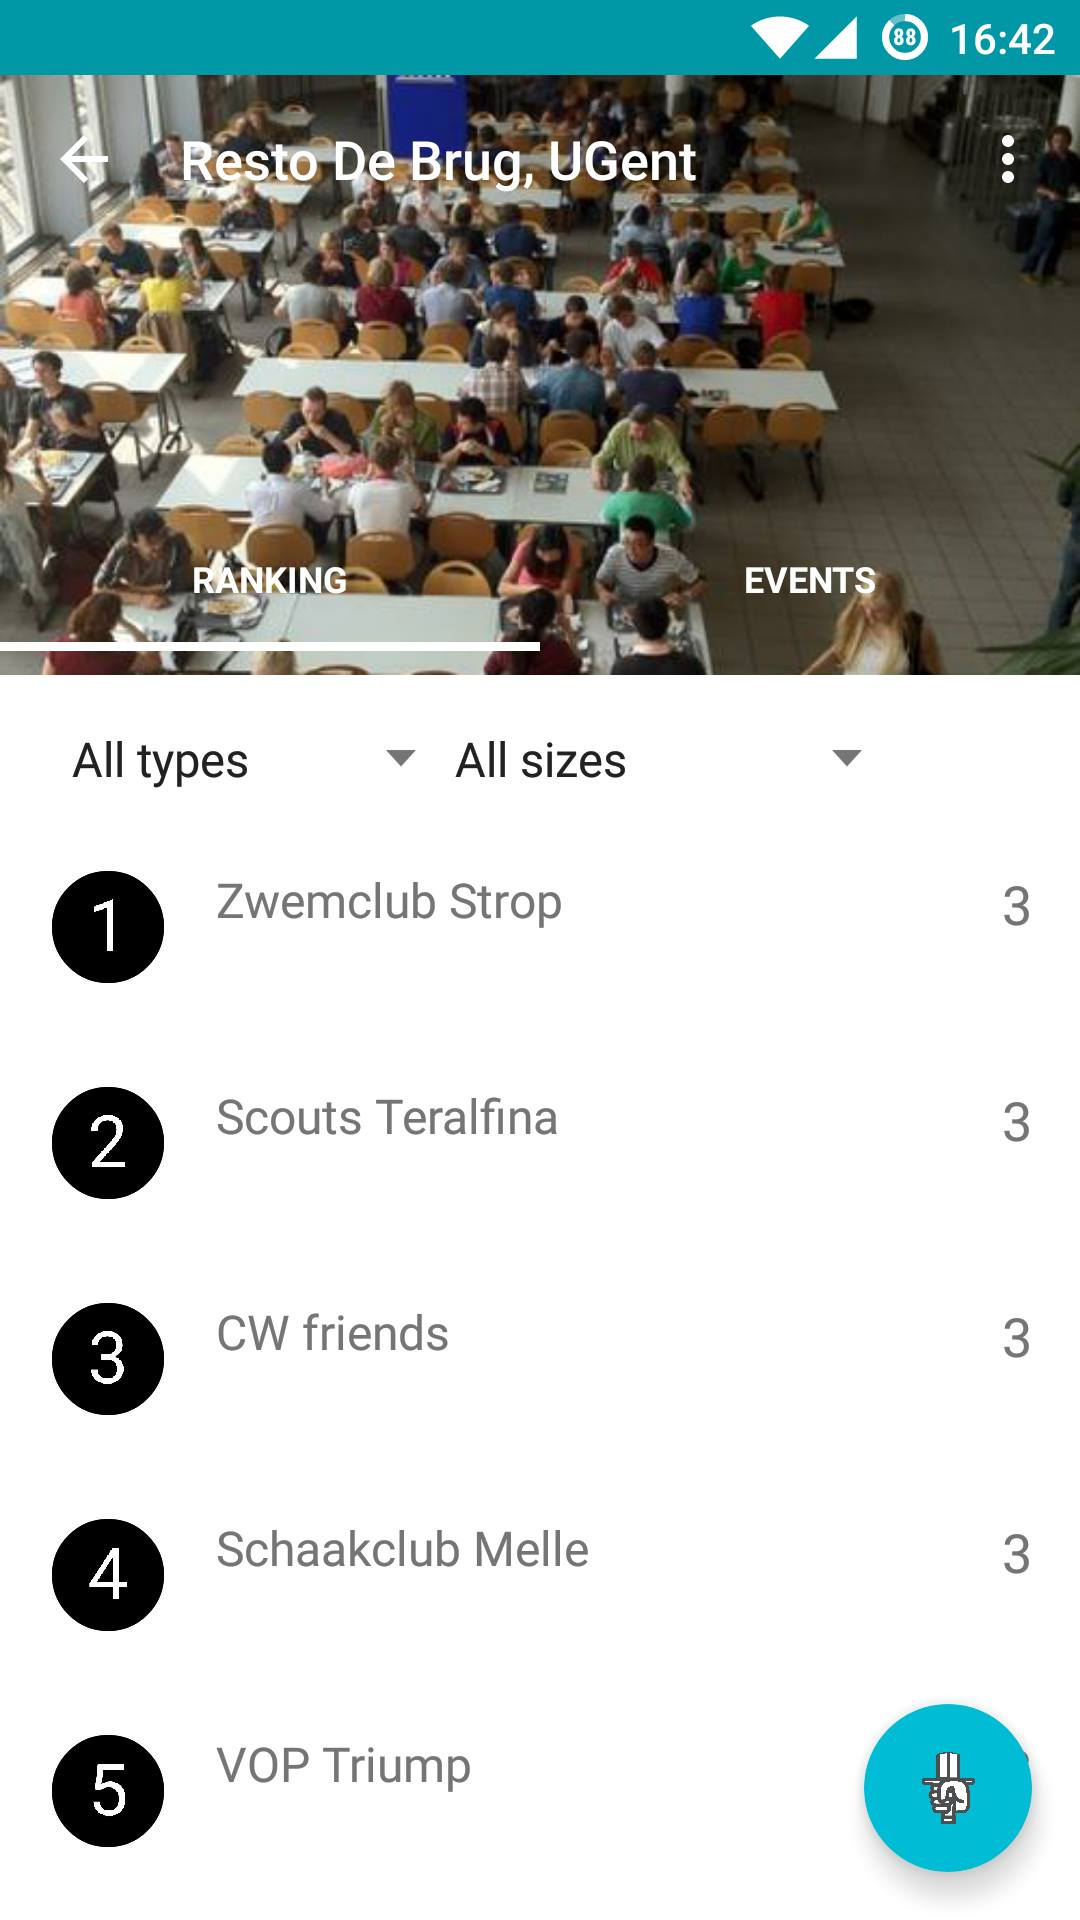
\includegraphics[width=\textwidth]{shot_venue}
\caption{Locatie}
\label{fig:screenshot_venue}
\end{minipage}
\end{figure}
\clearpage
\subsubsection{Groepen}%Lars
Een belangrijk onderdeel van de Triump applicatie is het groepsaspect. Groepen kunnen vanuit de toepassing zelf aangemaakt worden, en opgezocht worden. Daarnaast kunnen leden zich inschrijven voor groepen, en administrators kunnen deze aanvaarden. Vanop de startpagina kan de gebruiker de activiteit van groepsleden bekijken en navigeren naar zijn eigen groepen. Ranglijsten en evenementen steunen steeds op dit groepsprincipe in de zin dat de entiteiten waarvoor ranglijsten en evenementen opgesteld worden steeds groepen zijn. Dezelfde functionaliteit is ook mogelijk vanuit de webinterface (in het geval dat gebruik op de smartphone te onoverzichtelijk wordt).
Figuur \ref{fig:shot_groups} tot \ref{fig:shot_group} tonen de verschillende schermen met betrekking tot groepen.

\begin{figure}[ht]

\begin{minipage}[b]{0.25\linewidth}
\centering

\includegraphics[width=\textwidth]{shot_groups}
\caption{Groepen bekijken}
\label{fig:shot_groups}
\end{minipage}
\hspace{1cm}
\begin{minipage}[b]{0.25\linewidth}
\centering
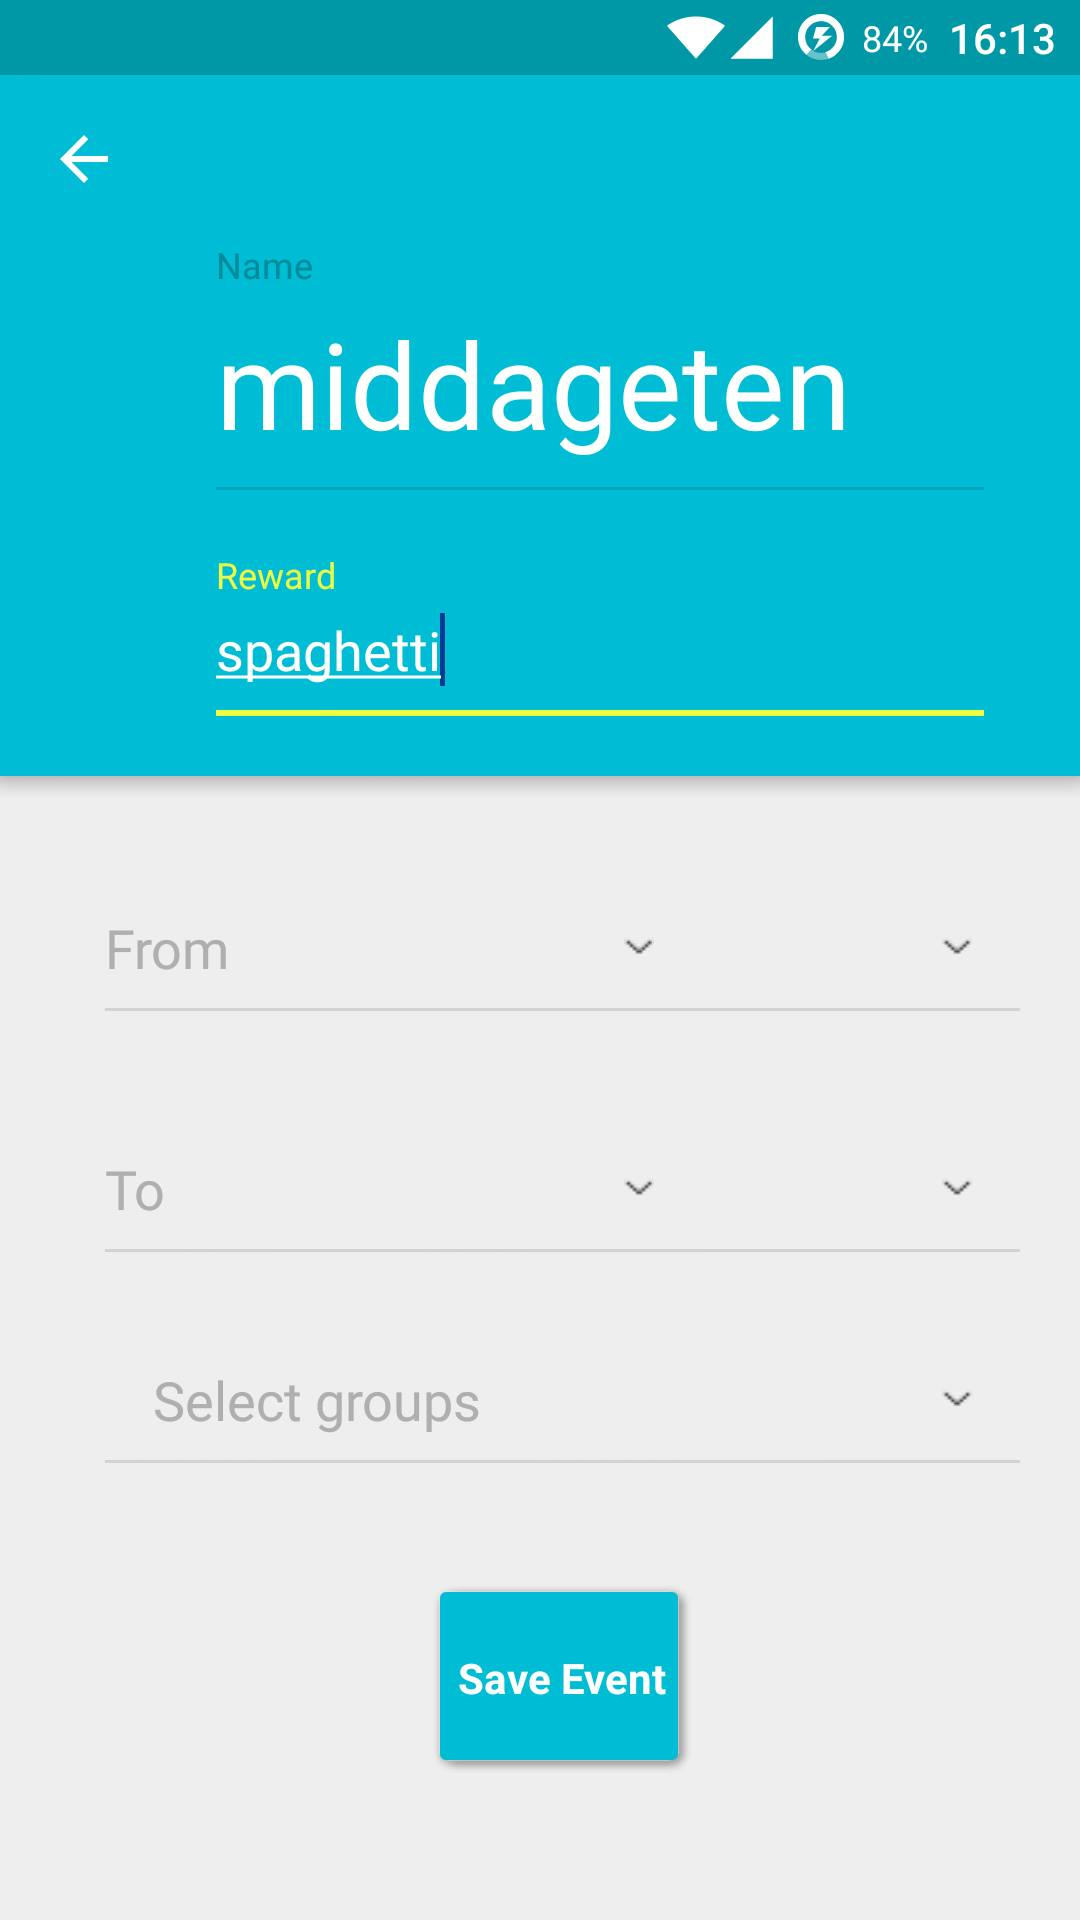
\includegraphics[width=\textwidth]{shot_groep_aanmaken}
\caption{Groep aanmaken}
\label{fig:shot_groep_aanmaken}
\end{minipage}
\hspace{1cm}
\begin{minipage}[b]{0.25\linewidth}
\centering

\includegraphics[width=\textwidth]{shot_group}
\caption{Groep-informatie}
\label{fig:shot_group}
\end{minipage}

\end{figure}

% % % % % % % % % % % % % % % % % % % % %
% afbeeldingen 2
\begin{figure}[ht]
\centering
\begin{minipage}[b]{0.5\linewidth}
\centering
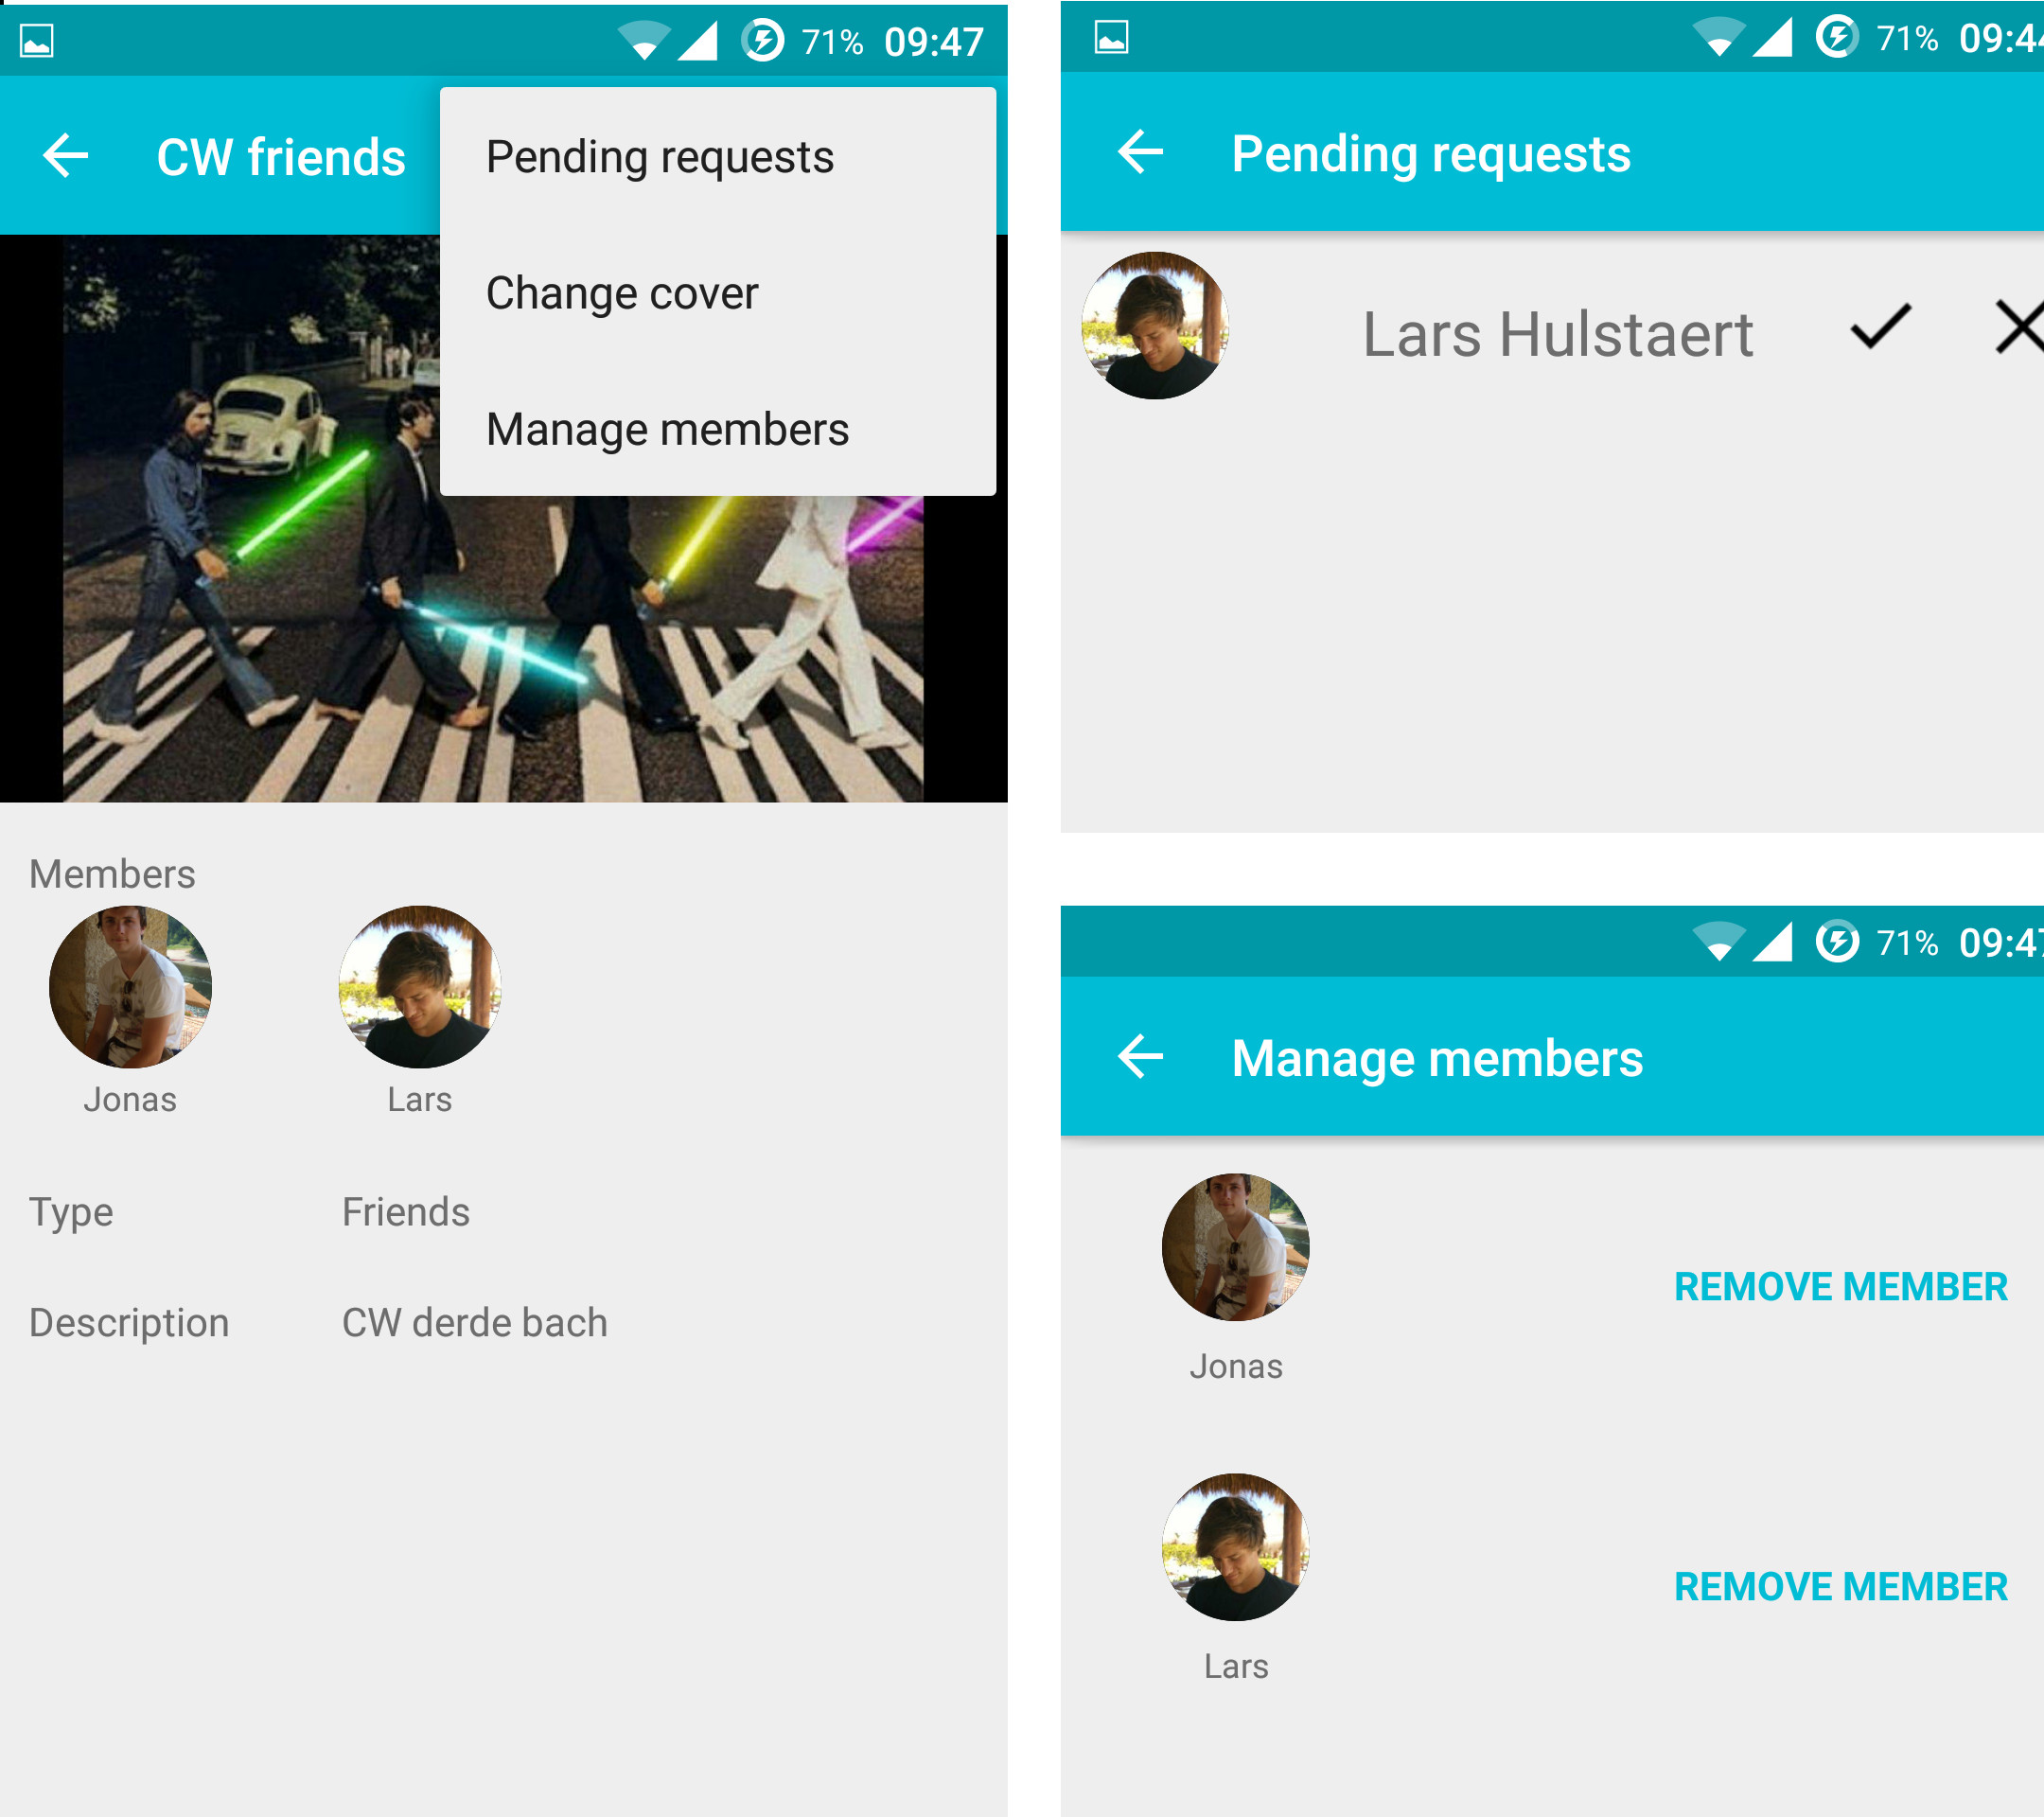
\includegraphics[width=\textwidth]{shot_groep_beheer}
\caption{Beheer groep. Accepteer lidschapverzoeken en verwijder leden}
\label{fig:shot_groep_beheer}
\end{minipage}


\end{figure}

\clearpage

\subsubsection{Events en Rewards}%Siebe
Op een bepaalde locatie kan een gebruiker een evenement aanmaken (Fig. \ref{fig:shot_event_aanmaken}).
In het Eventsscherm (Fig. \ref{fig:shot_event}) krijgt de gebruiker een overzicht van alle evenementen. Hierbij worden officiële en niet-officiële in dezelfde lijst weergegeven maar worden ze grafisch onderscheiden. Het Eventsscherm is geïmplementeerd om te vermijden dat gebruikers via de locaties op zoek moet gaan naar evenementen.
In het Rewardscherm (Fig. \ref{fig:shot_reward_claim}) kan de gebruiker de promoties van officiële evenementen gaan opeisen indien hij/zij deze heeft gewonnen met één van zijn groepen. Momenteel kan de gebruiker beloningen opeisen door over een promotie te vegen, waarbij een dialoogscherm wordt geopend. Door dit scherm aan de eigenaar te tonen, kan vervolgens de beloning geïnd worden. Als uitbreiding kan er eventueel voor gezorgd worden dat de eigenaar een unieke afbeelding uploadt per promotie. Door te vegen over de promotie kan de afbeelding dan bv. 10 s getoond worden.
\subsubsection{Leaderboard}%Lars
Het Leaderboardscherm toont een algemene ranglijst. Deze ranglijst is onafhankelijk van een locatie en toont welke groepen zich globaal aan de leiding bevinden op basis van het aantal checkins. Momenteel wordt deze ranglijst nog in hetzelfde formaat getoond als bij de locaties. Een mogelijke uitbreiding is echter om naast een lijst te tonen, ook een kaartje te tonen dat dynamisch gegenereerd. Deze kaart zou dan per locatie tonen welke groep hier aan de leiding staat. De Leaderboards kunnen gewijzigd worden afhankelijk van grootte en type van de groepen. Het Leaderboardscherm is gebaseerd op hetzelfde concept als de ranglijsten van Fig. \ref{fig:screenshot_venue}.
\subsubsection{Notificaties} %Vincent
Het notificatiesysteem zorgt ervoor dat gebruikers verwittigd worden van belangrijke gebeurtenissen binnen Triump en met slechts één beweging de betreffende pagina kunnen waarnemen. In de huidige implementatie zal een gebruiker een notificatie ontvangen indien een groep waartoe hij/zij behoort een evenement heeft gewonnen. Wanneer er op de notificatie wordt geklikt zal de evenementpagina meteen worden getoond. Daarnaast kan een gebruiker ook via notificaties aangespoord worden om feedback te verschaffen.   

\begin{figure}[ht]

\begin{minipage}[b]{0.25\linewidth}
\centering
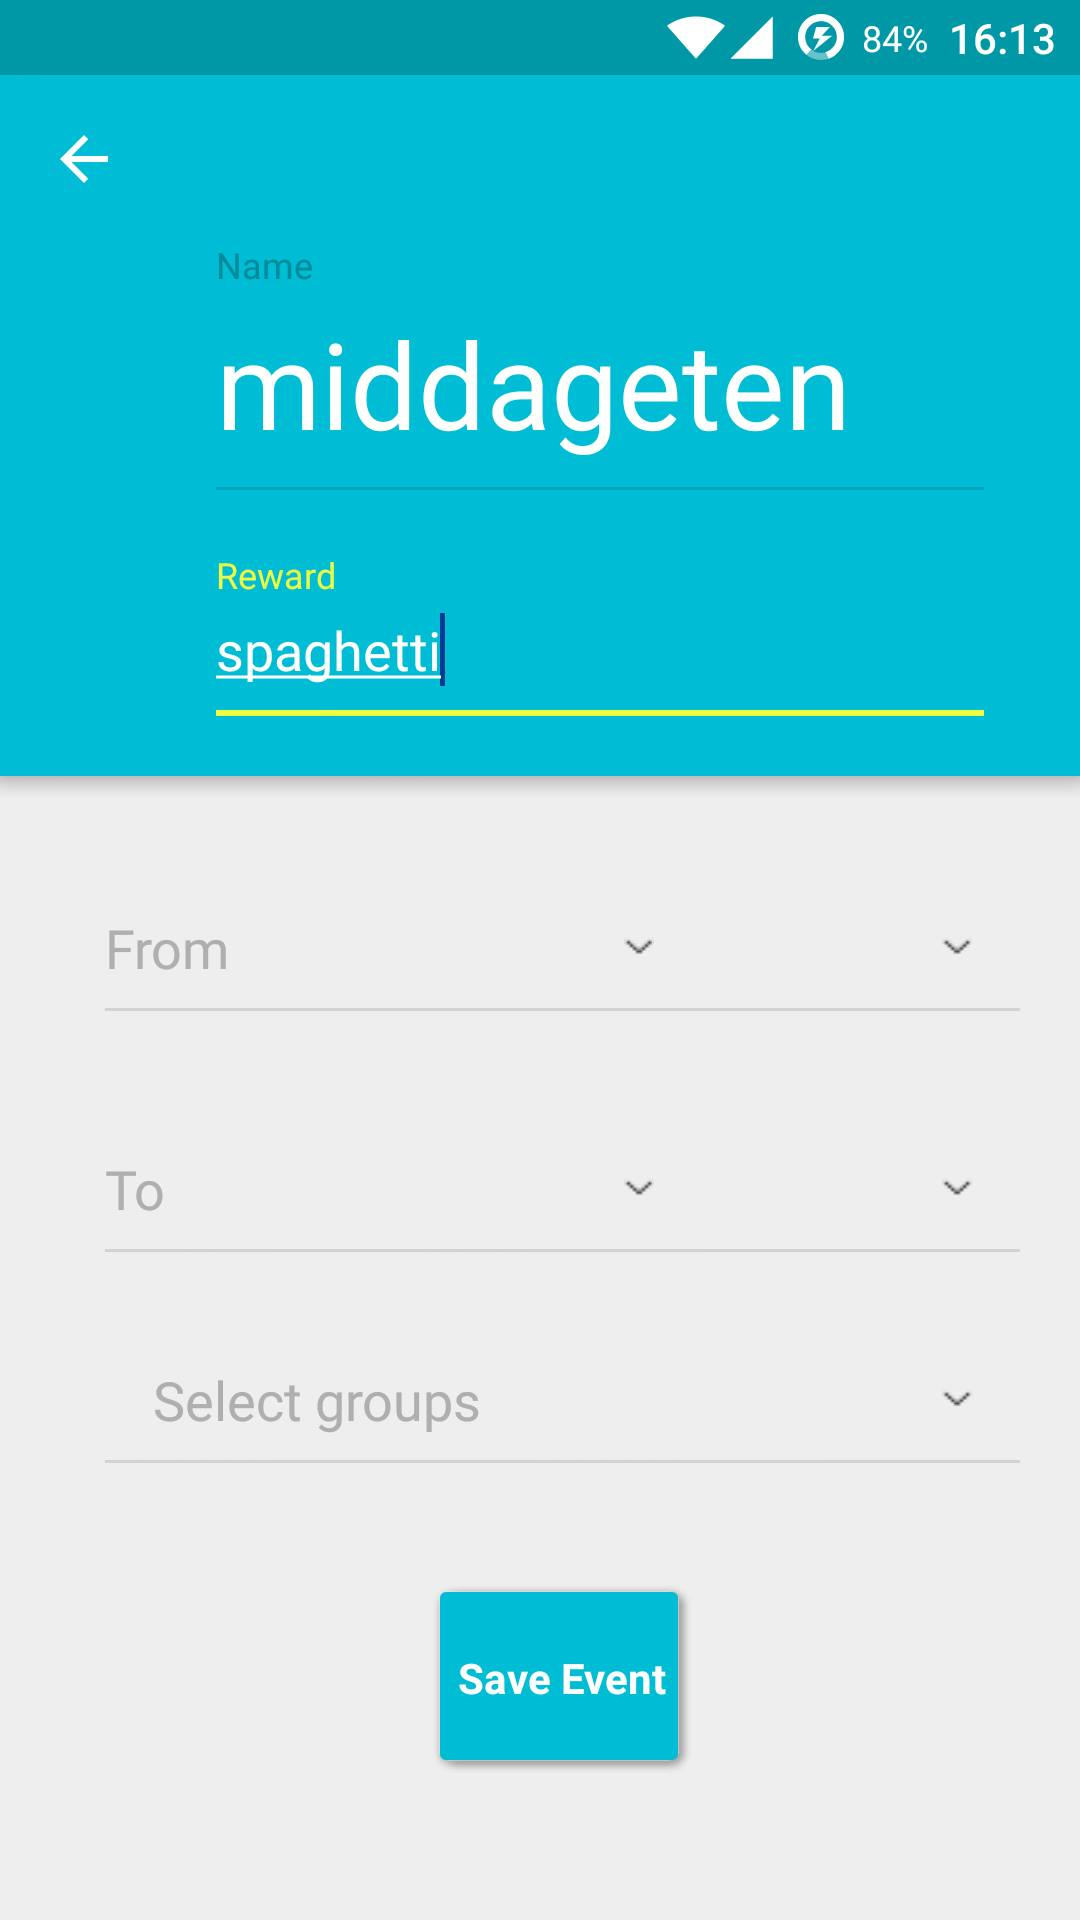
\includegraphics[width=\textwidth]{shot_event_aanmaken}
\caption{Event aanmaken}
\label{fig:shot_event_aanmaken}
\end{minipage}
\hspace{1.8cm}
\begin{minipage}[b]{0.25\linewidth}
\centering
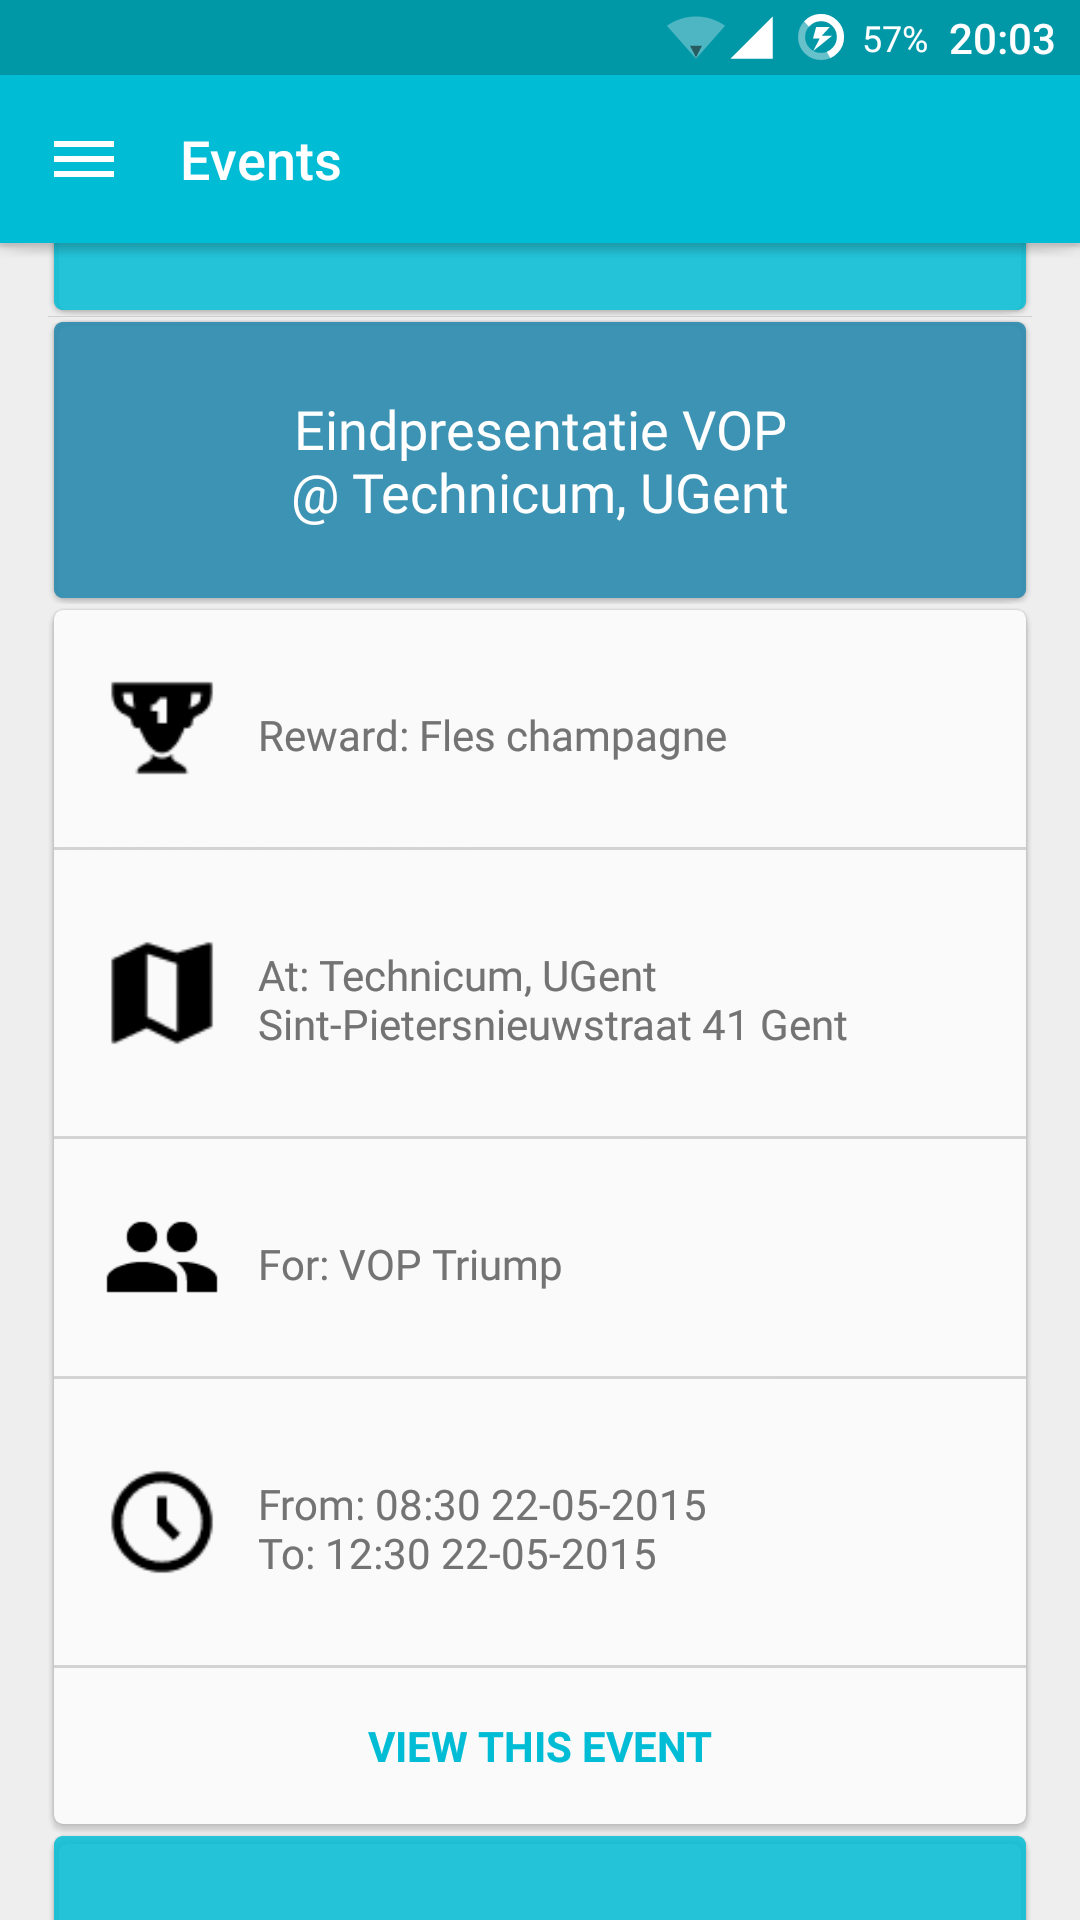
\includegraphics[width=\textwidth]{shot_event}
\caption{Event-informatie}
\label{fig:shot_event}
\end{minipage}
\hspace{1.8cm}
\begin{minipage}[b]{0.25\linewidth}
\centering
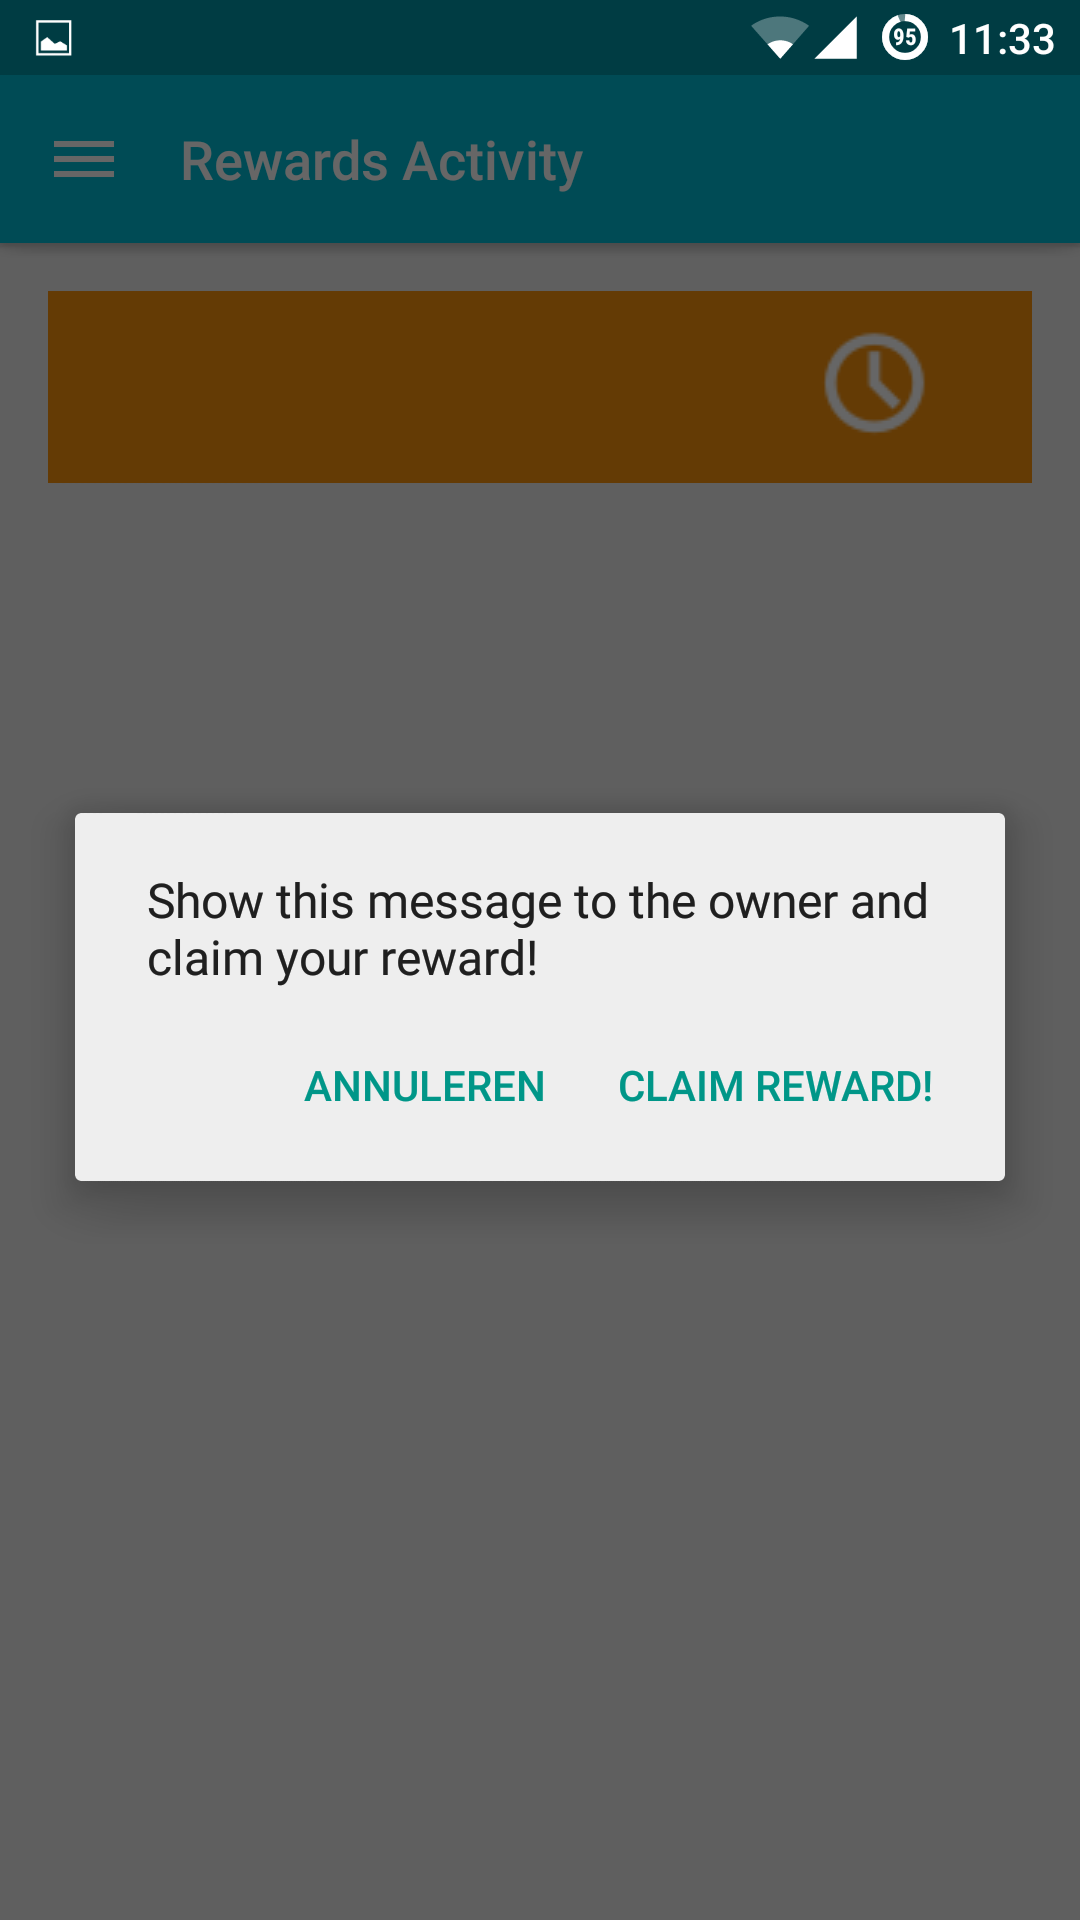
\includegraphics[width=\textwidth]{shot_reward_claim}
\caption{Ontvang promotie}
\label{fig:shot_reward_claim}
\end{minipage}
\end{figure}
\clearpage

\subsubsection{Feedback}%Siebe
In de ontwikkelfase, maar ook bij het uitbrengen van een eerste versie van de toepassing is feedback van cruciaal belang. Om het testgebruikers mogelijk te maken vanuit de applicatie zelf feedback te laten geven wordt een Feedbackscherm voorzien (Fig. \ref{fig:shot_feedback}). De gebruiker kan in een tekstveld schrijven wat hij van Triump vindt en eventuele bugs melden. Deze berichten worden dan onmiddelijk doorgestuurd naar het gemeenschappelijk emailadres van Triump.
\subsubsection{Settings en profile}% Lars
Om de applicatie configureerbaar te maken wordt een instellingscherm voorzien (Fig. \ref{fig:shot_instellingen}). Hiervoor wordt de methode voorzien voorgeschreven door Google Applications.
Voorbeelden van instellingen in Triump zijn: het aan- en uitzetten van notificaties, het al dan niet delen van je profiel, het kleurenschema dat de applicatie gebruikt,... 
In Figuur \ref{fig:shot_profile} wordt het persoonlijk profiel getoond, waarbij reeds verwezelijkte doelstellingen (achievements) worden getoond. 

\begin{figure}[ht]

\begin{minipage}[b]{0.25\linewidth}
\centering
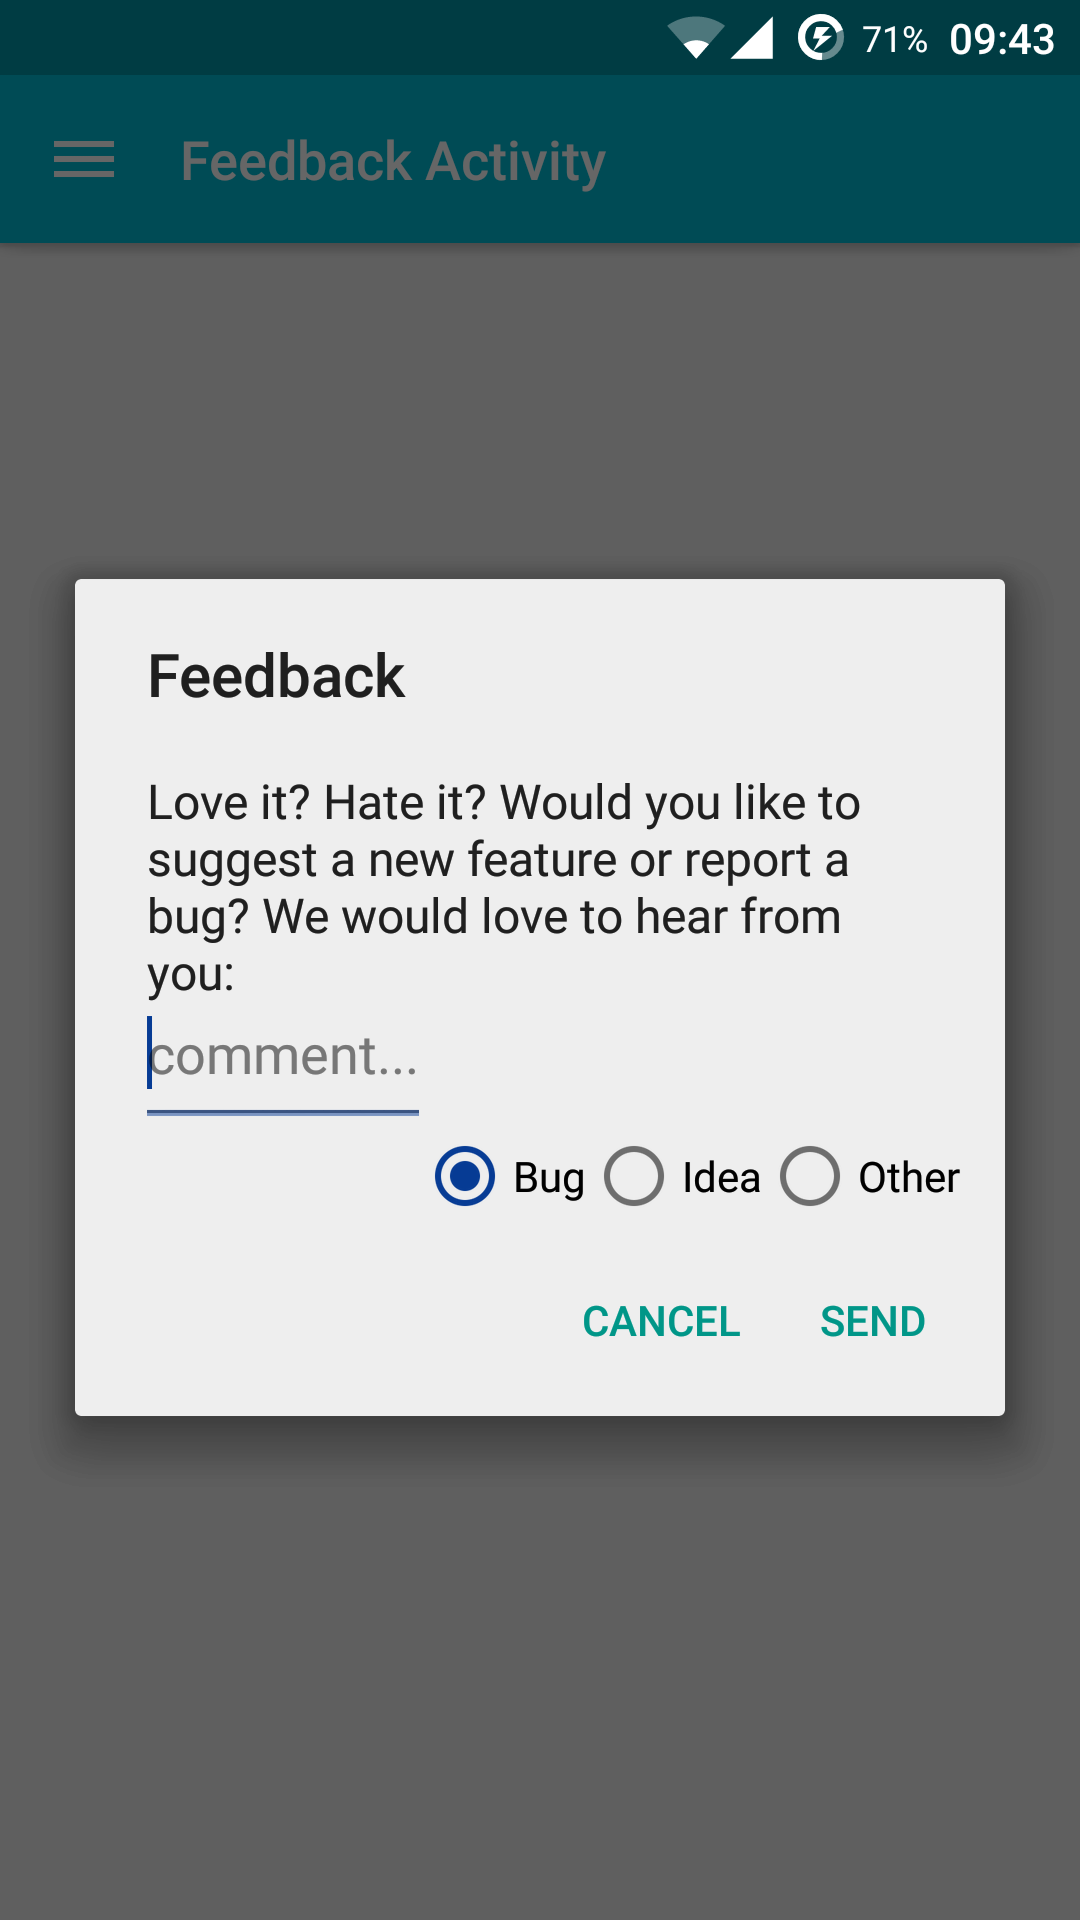
\includegraphics[width=\textwidth]{shot_feedback}
\caption{Feedback}
\label{fig:shot_feedback}
\end{minipage}
\hspace{1.5cm}
\begin{minipage}[b]{0.25\linewidth}
\centering
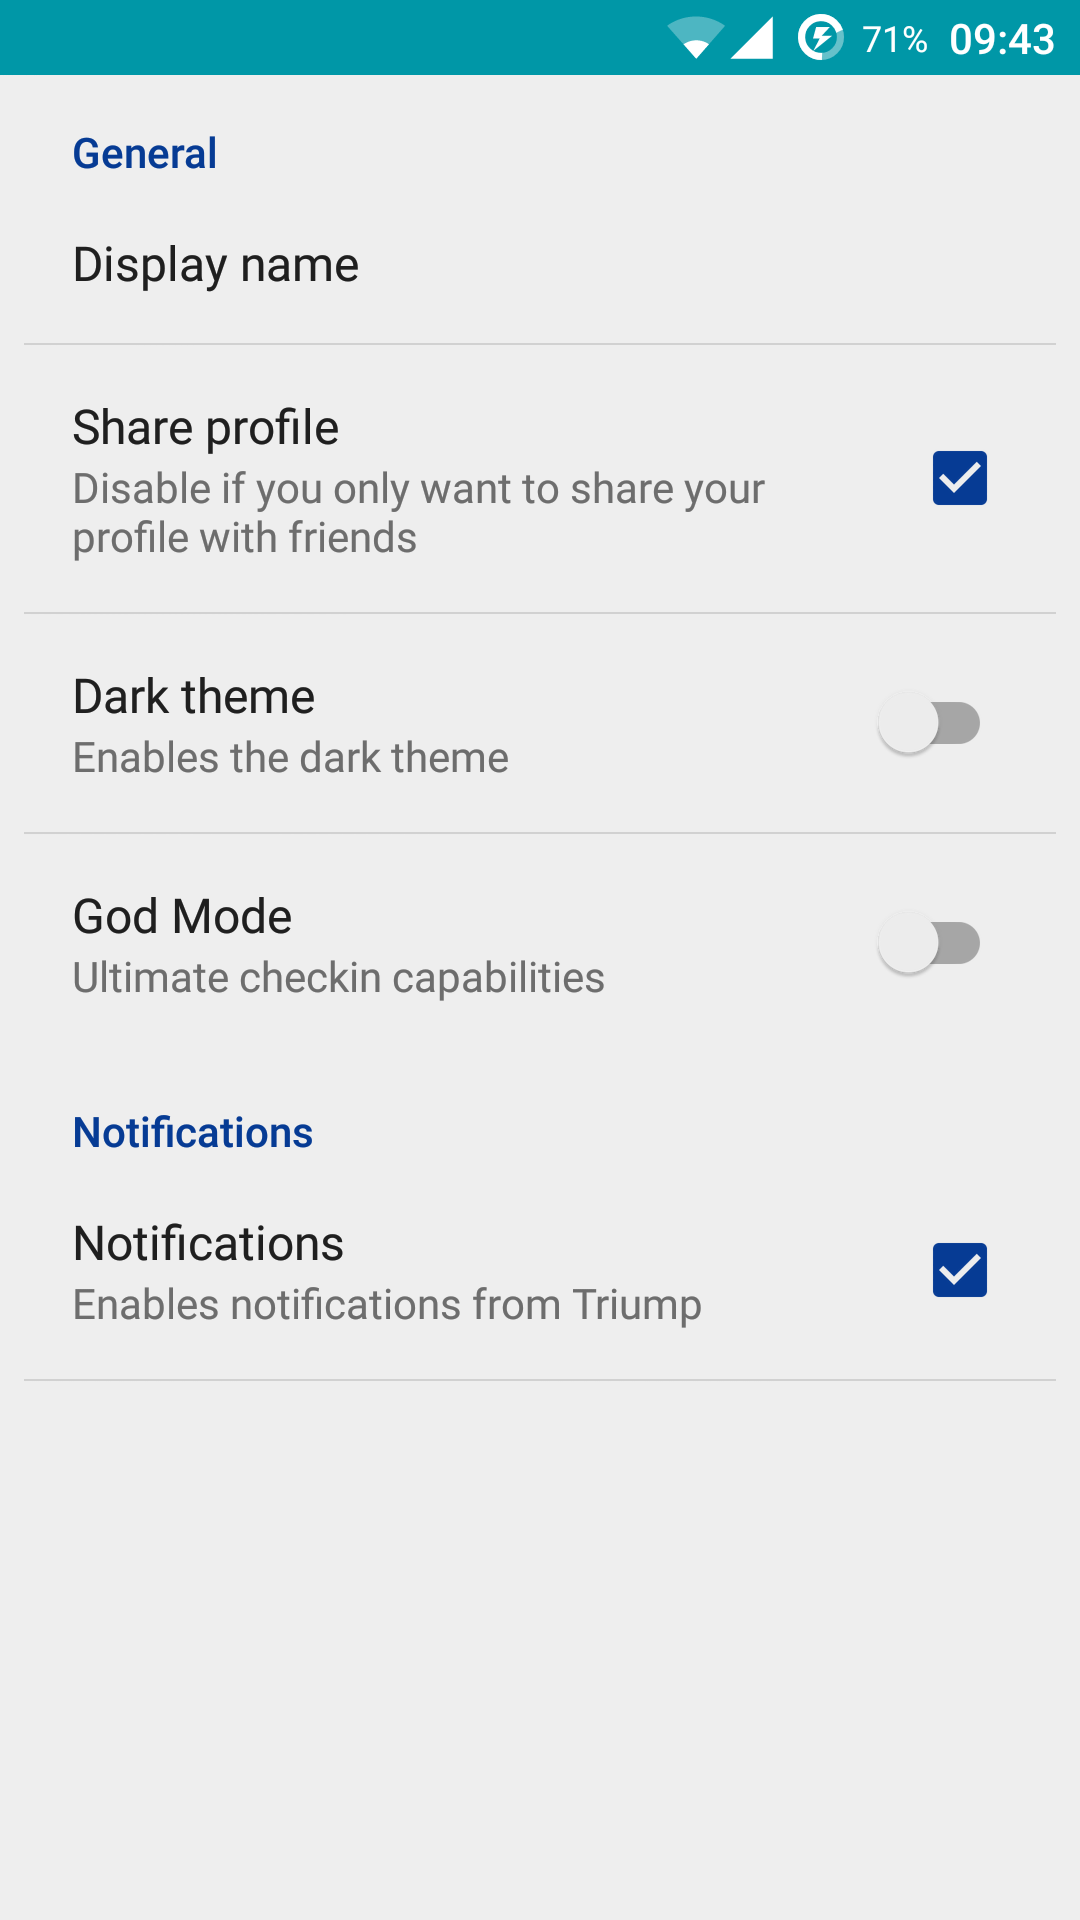
\includegraphics[width=\textwidth]{shot_instellingen}
\caption{Instellingen}
\label{fig:shot_instellingen}
\end{minipage}
\hspace{1.5cm}
\begin{minipage}[b]{0.25\linewidth}
\centering
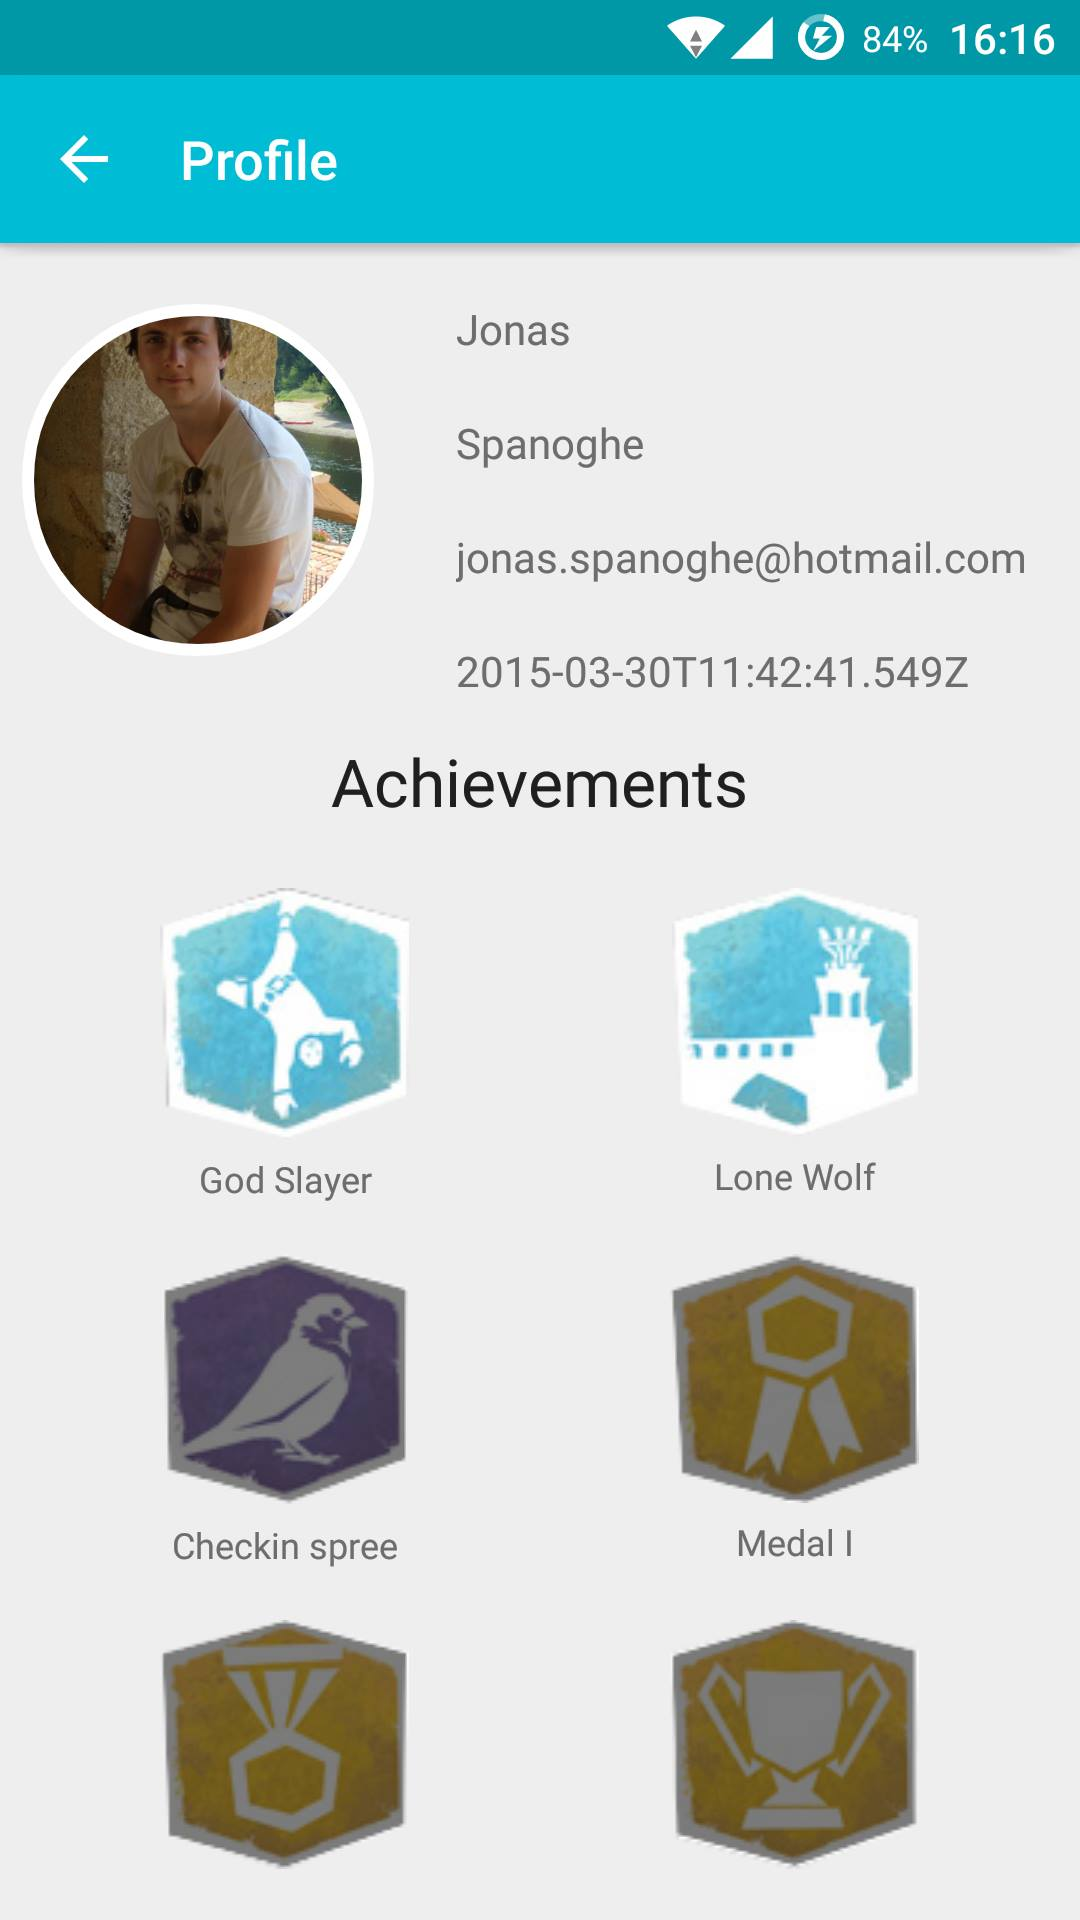
\includegraphics[width=\textwidth]{shot_profile}
\caption{Profiel}
\label{fig:shot_profile}
\end{minipage}
\end{figure}

\section{Webinterface}%Jonas -A
De website van Triump, die te bekijken is op triump.be, bestaat uit 2 delen. Enerzijds is er een deel waarvoor men niet dient ingelogd te zijn. Hier kan men informatie vinden over Triump, de applicatie downloaden en de ontwikkelaars contacteren . Anderzijds is er de interface voor gebruikers van Triump, waarvoor men ingelogd dient te zijn. Hier kan men groepen en evenementen bekijken, maar de belangrijkste functionaliteit van dit gedeelte is het registreren van een locatie.
Het registreren van een locatie is noodzakelijk indien men een officieel evenement wil organiseren.
\subsubsection{Publieke pagina's}
De publieke pagina's van de website ( Fig. \ref{fig:about}) zijn voornamelijk bedoeld ter promotie van Triump. Vanuit de startpagina kan genavigeerd worden naar `Contact' en `About' om meer informatie over Triump te verkrijgen. Via de sectie `Download' kan de applicatie gedownload worden. Dit is voornamelijk bedoeld voor de testgebruikers, vermits lancering op de Google App Store pas na uitvoerig testen mogelijk is. Testgebruikers kunnen de testversie downloaden via de website. Via `Sign up' kunnen gebruikers zich registreren om gebruik te kunnen maken van de webinterface voor Triump.\\
Op de Contact-pagina is er de mogelijkheid om feedback te geven en een mail te sturen.
Op de About-pagina vindt men algemene informatie over de applicatie.
\subsubsection{Inloggen}
Om de webinterface van Triump te kunnen gebruiken, dient men zich eerst te registreren. Hierna logt men dan in met de nieuwe account die men kan koppelen aan Foursquare ( Fig. \ref{fig:events}).
\subsubsection{Registreren van locatie}
Nadat men is ingelogd kan men een locatie uit de Foursquare-database bij Triump registreren.
Momenteel is het enkel mogelijk om te zoeken naar locaties rondom Gent, aangezien de eerste testen van Triump daar gebeuren.
Om er zeker van te zijn dat het wel degelijk om de juiste locatie gaat, is er een link aanwezig die leidt naar de Fourquare-pagina van die locatie.
Vervolgens bevestigt de gebruiker de registratie en wordt een mail te gestuurd naar Triump met de details van de locatie. De registratie wordt geverifieerd en uiteindelijk goedgekeurd.
De gebruiker kan vervolgens een officiëel evenement organiseren voor deze locatie via de webinterface.
\begin{figure}[H]
	\centering
	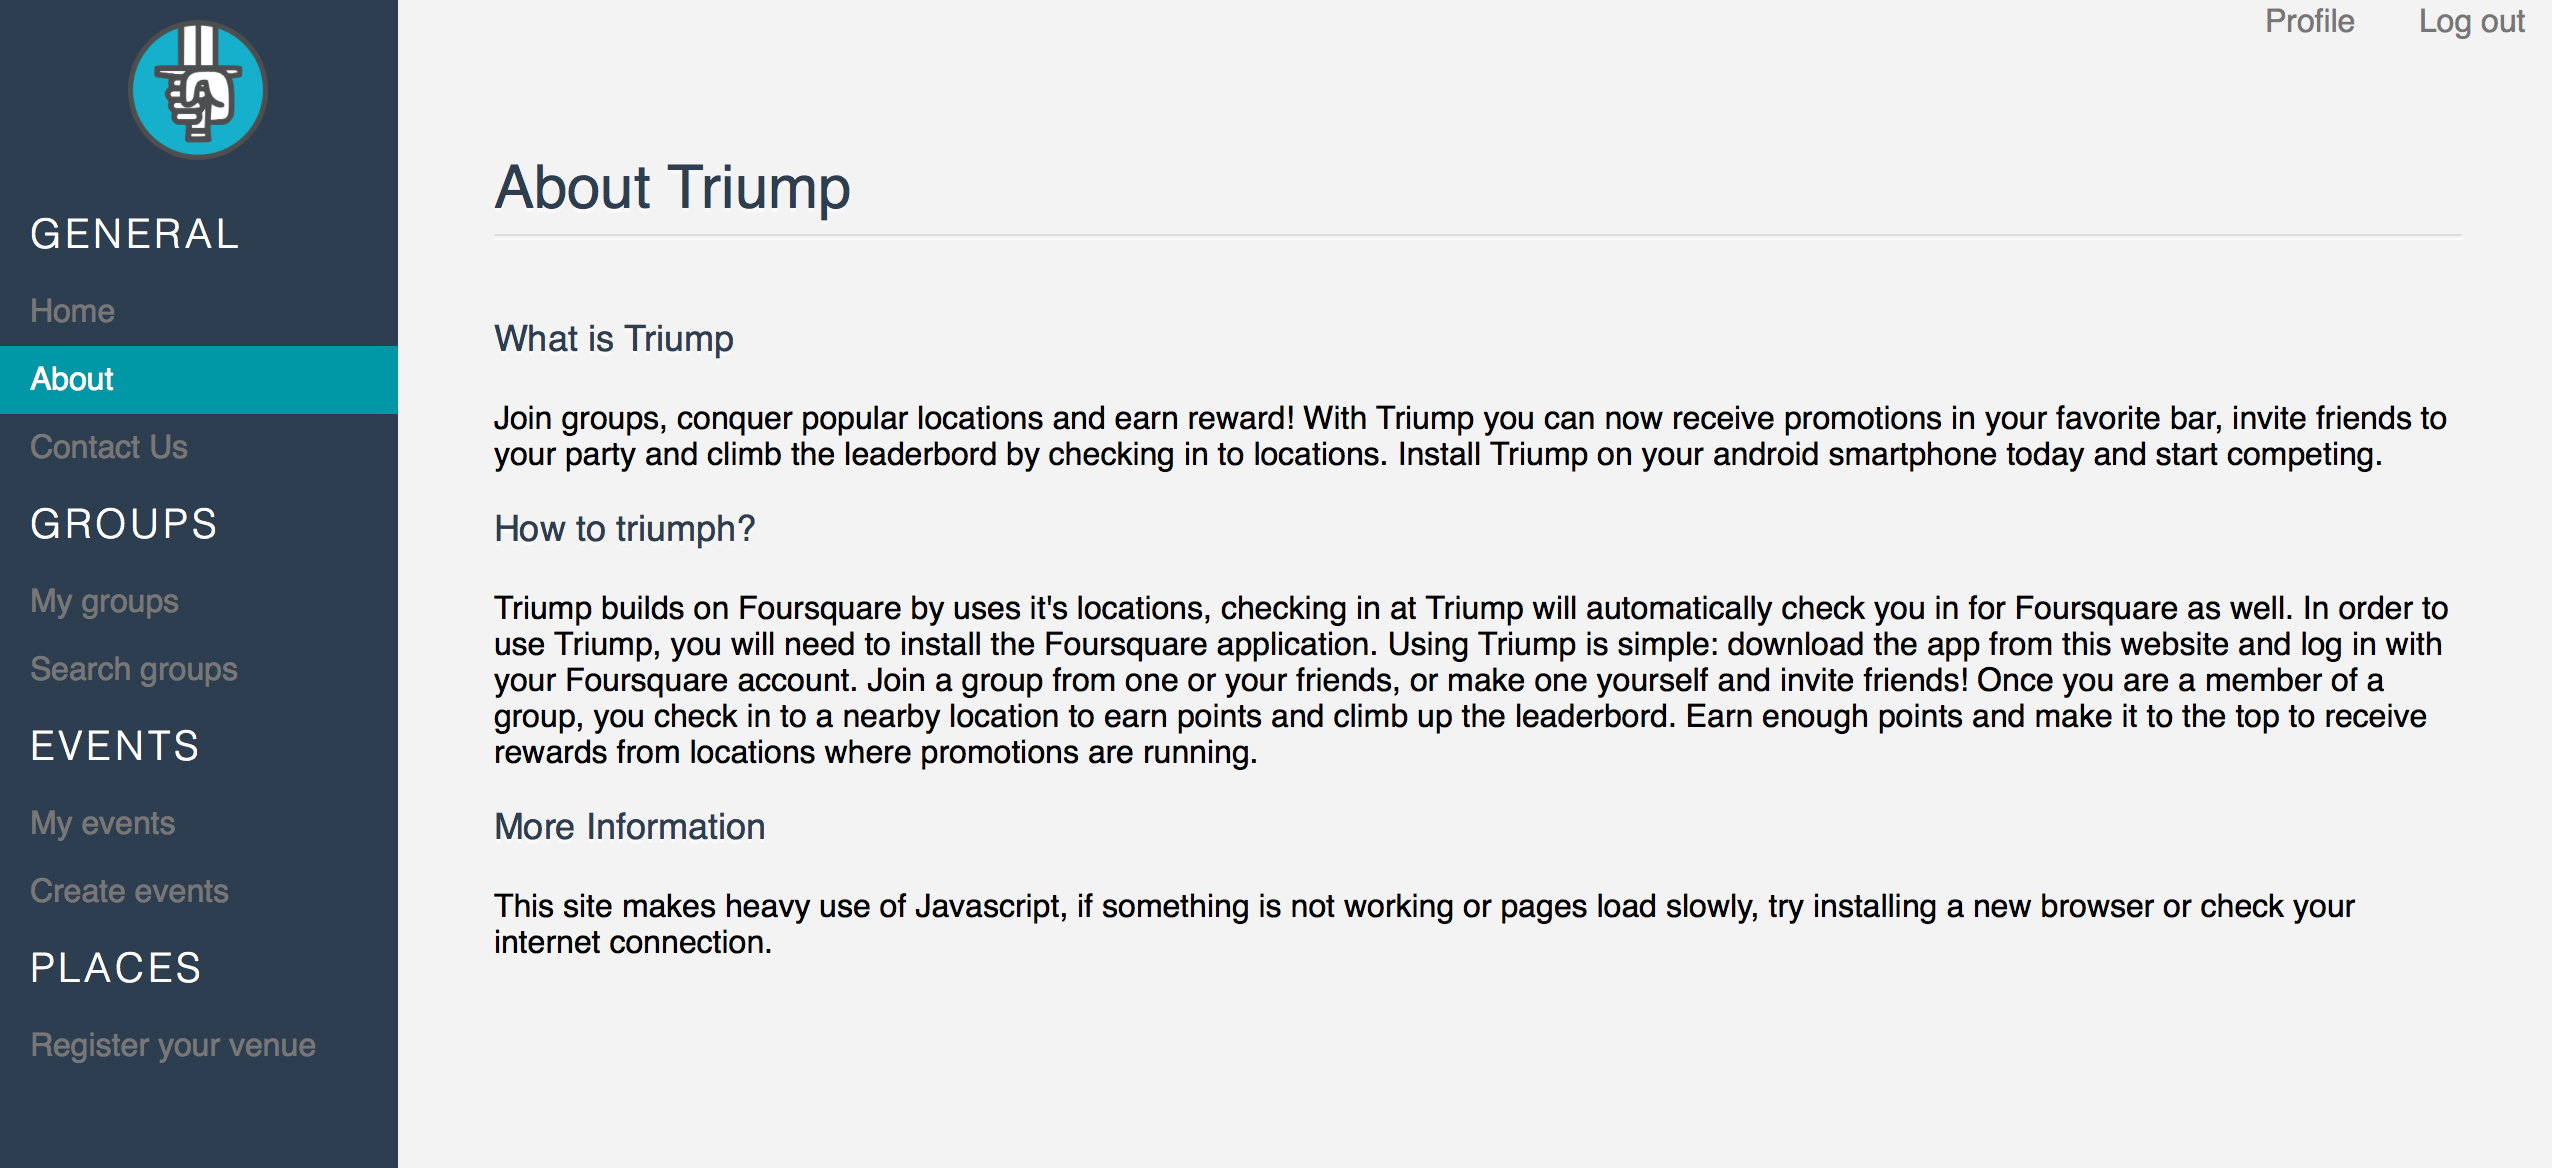
\includegraphics[scale=0.3]{about}
	\caption{Publieke website }
	\label{fig:about}
\end{figure}

\begin{figure}[H]
	\centering
	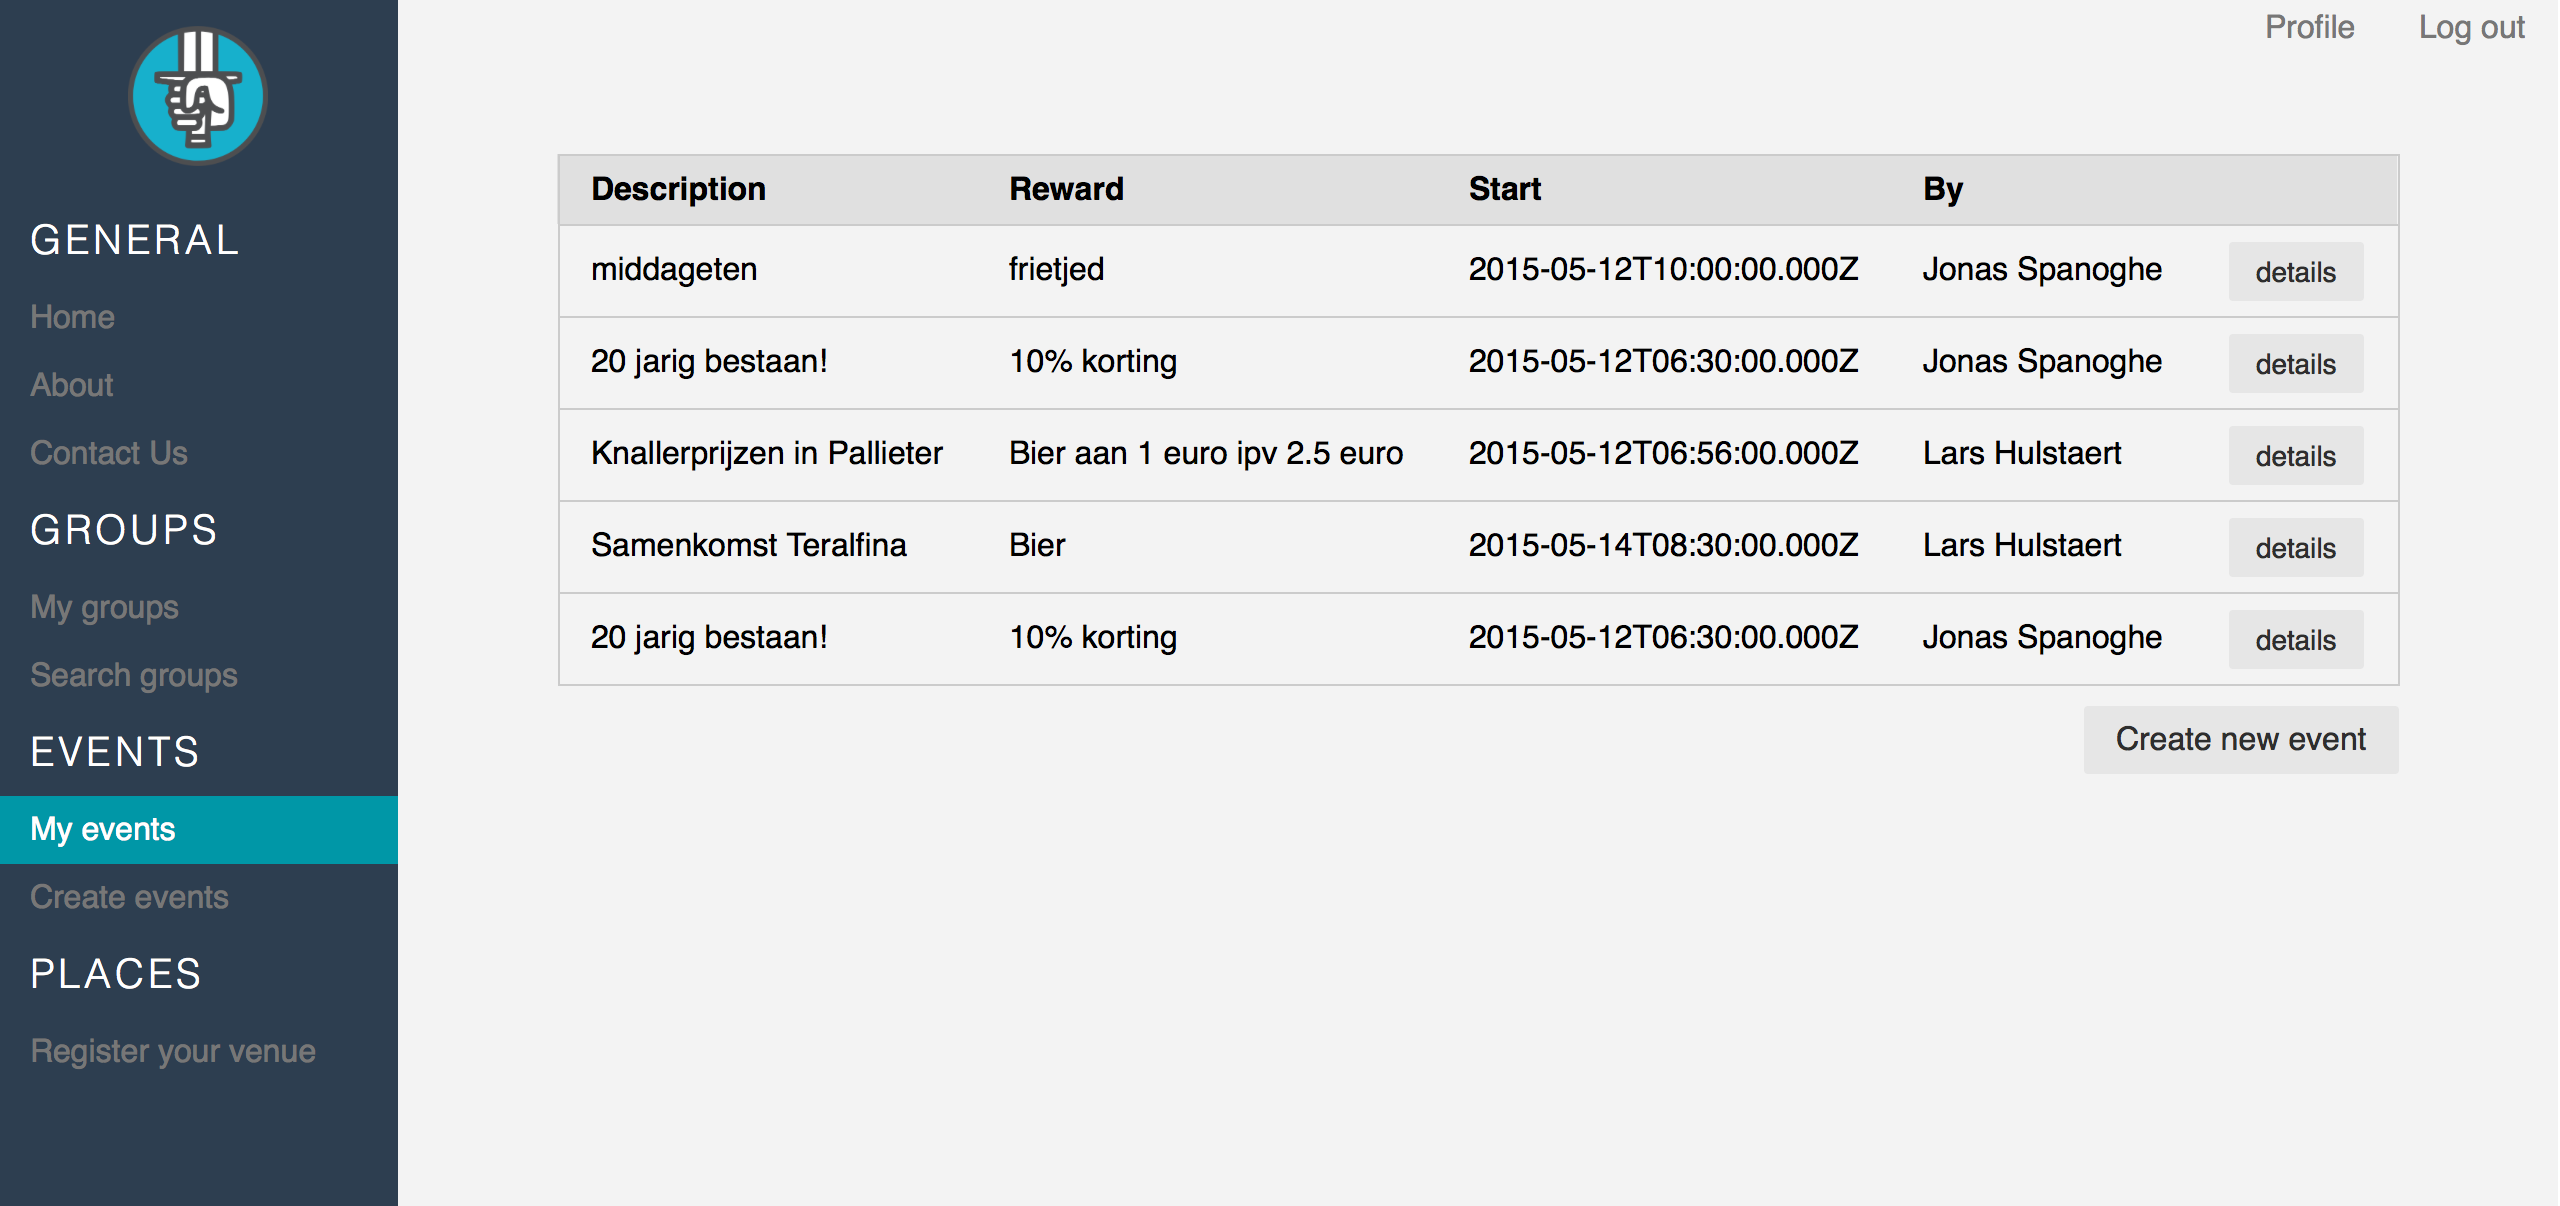
\includegraphics[scale=0.3]{events}
	\caption{Webinterface }
	\label{fig:events}
\end{figure}

% Verschillende schermen tonen van webinterface en functionaliteit

\chapter{Testen}

%Een overzicht van de testen en testmogelijkheden die werden ingebouwd of
%uitgevoerd.


% Backend testen, statistieken over de endpoints
% Userfeedback: Integratie van feedbacksysteem om gebruikervaringen bij te houden.

\chapter{Groepsdynamiek} %Vincent

% Een bespreking van de samenwerking, organisatie en communicatie
% binnen de groep.



\chapter{Analyse van de openstaande problemen}%Lars

% Analyse van de openstaande problemen, tekorten, eventuele foute beslissingen
\section{Tijdsduur backend API Calls}
\label{tijdsduur}
Zoals aangehaald in sectie \ref{sec: GCE} Google Cloud Endpoints is een van de nadelen van GCE de grote variatie in tijdsduur van backend API calls. Figuur \ref{fig:hist_getAllGroups} is een histogram die de relatieve frequentie weergeeft van de tijdsduur van een bepaalde API call; gelijkaardige histogrammen worden bekomen voor andere API calls. De histogram is gebaseerd op 26 meetpunten verspreid over 2 dagen. GCE houdt een bepaalde backend instantie niet continu in ingeladen op de servers. De grote variatie in de tijden is m.a.w. te wijten aan het opstarten van de instantie. Deze wachttijden hebben een negatieve impact op de gebruikerservaring. Indien de toepassing echter meer wordt gebruikt, is de backend instantie meer actief en vormen `koude missers' minder een probleem.
\begin{figure}[H]
	\centering
	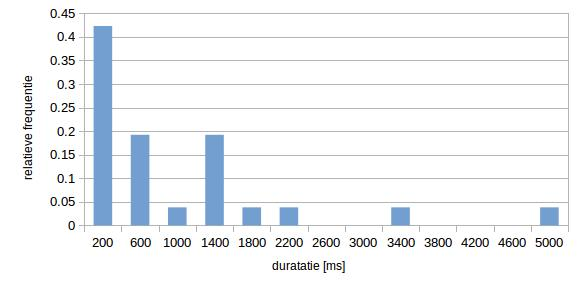
\includegraphics[scale=0.5]{prestatie_histogram_GCE}
	\caption{Histogram tijdsduur methode oproep getAllGroups()}
	\label{fig:hist_getAllGroups}
\end{figure}


\section{Checkin entiteiten}

In de huidige implementatie van de backend API wordt er voor iedere checkin van een gebruiker en voor iedere groep waartoe de gebruiker behoort een checkin entiteit aangemaakt. Hierdoor groeit het aantal entiteiten in de Checkin tabel zeer snel. Daarnaast komt nog dat Triump gebruik maakt van GAE Datastore voor de backend database. Bij het gebruik van deze Datastore horen quota's die beperkingen opleggen voor de grootte van de databank en voor het aantal entiteiten. 
% Hier moet een afbeelding komen:
% Grafiek van percentage types in datastore ...
De eenvoudigste oplossing voor dit probleem is het uitbreiden van de datastore door een dagelijks bedrag te betalen aan GAE. Een andere oplossing is het opstarten van een periodieke Cron job (zie sectie \ref{sec: GCE} Cron jobs) die bijvoorbeeld wekelijks de Checkin tabel `samenvat'. De samenvatting kan gebeuren door alle punten verzamelt door 1 groep op 1 locatie binnen een bepaalde periode toe te kennen aan 1 checkin entiteit. Op deze manier kan het aantal entiteiten drastisch beperkt worden. Nadeel van deze oplossing is het verlies aan informatie die mogelijks gebruikt kan worden voor het genereren van statistieken. 

Aangezien de opgelegde quota's m.b.t. de GAE Datastore ruimschoots voldoen en bijgevolg het probleem nog niet van toepassing is, zijn nog geen van beide oplossingen geïmplementeerd.
Indien het aantal gebruikers van Triump zou toenemen is het wel noodzakelijk een oplossing toe te passen.

\section{Android versies}

Android is een besturingssysteem waaraan continu wordt gesleuteld door Google. Er worden met regelmaat verbeteringen en wijzigingen doorgevoerd, en dit resulteert in verschillende versies van Android.
Op Figuur \ref{fig:android_versions} kan men zien dat op het moment van schrijven voornamelijk Android versies 4.0 en later worden gebruikt. Deze worden ondersteund in Triump, om een zo groot mogelijk doelpubliek te hebben. Het ondersteunen van verschillende versies brengt echter ook moeilijkheden met zich mee. Vaak worden samen met een nieuwe versie van Android, ook nieuwe concepten uitgebracht.
Een voorbeeld hiervan is de `CardView' en `Material Design' uit de laatste versie, Lollipop. Er is `backward compatability' voorzien voor vorige versies van Android, maar daarop worden o.a. de `Cards' minder mooi weergegeven.
Ook is er een enorme diversiteit aan schermen van smartphones. Deze verschillen sterk in grootte en resolutie, wat ervoor zorgt dat het moeilijk is een layout te maken die op alle schermen even duidelijk en mooi overkomt.
Verder heeft Google sinds Lollipop regels opgelegd over hoe een moderne applicatie het best visueel wordt ontworpen, genaamd `Material Design'. Het grootste probleem dat wij hiermee ondervonden was het feit dat wel werd vertelt `wat' er moest gebeuren, maar niet `hoe'. Details over de manier waarop de designrules moeten worden geïmplementeerd, zijn vrijwel nergens te vinden. Toch werd geprobeerd om deze opgelegde regels zo strikt mogelijk te volgen.
\begin{figure}[H]
	\centering
	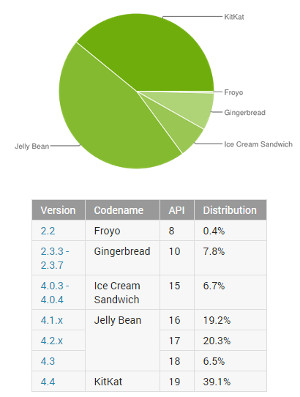
\includegraphics[scale=0.27]{android-versions}
	\caption{distributie van de Android versies in het begin van 2015}
	\label{fig:android_versions}
\end{figure}

\section{Batterijgebruik en efficiëntie}
Momenteel verbruikt de Android applicatie veel energie omdat continu gegevens opgevraagd worden over het netwerk. Ook de locatie van de gebruiker wordt frequent opgevraagd.
Een oplossing voor dit probleem is o.a. caching van gegevens en geofencing. Wanneer een gebruiker informatie opvraagt kan een lokaal opgeslagen versie van het resultaat getoond worden. In 1 oproep naar de backend kan gecontroleerd worden of nieuwe informatie voor handen is. Indien dit het geval is, kunnen de laatste gegevens binnengehaald worden van de servers. Deze oplossing wordt reeds toegepast op informatie over locatie- en overzichtelementen. Als cache of lokale databank wordt een SQLite database gebruikt. Dit systeem wordt aangeboden door Android. Caching van alle data zoals de oplossing voorstelt is nog niet geïmplementeerd wegens het beperkte tijdskader van het vakoverschrijdend project.
Geofencing is een manier voor locatiegebaseerde applicaties om te verhinderen dat continu locatiegegevens via GPS opgevraagd dienen te worden. Deze oplossing werd uitvoerig bestudeerd, maar kon wegens tijdsgebrek niet in de eindoplossing opgenomen worden.




\chapter{Besluit}%Jonas

In dit vakoverschrijdend project werd een applicatie ontwikkeld, gericht op het uitbreiden van de functionaliteit van Foursquare en Qustomer.
Met Triump kunnen gebruikers zich verenigen in groepen en in competitie treden met andere groepen via de checkin functionaliteit van Foursquare.
Verder kunnen gebruikers evenementen aanmaken, waaraan een promotie kan gekoppeld worden. Zo kunnen uitbaters van bepaalde locaties Triump gebruiken om aan online marketing te doen.\\


Triump bestaat uit drie grote delen.
Er is de Android applicatie voor de traditionele gebruiker. Hiermee kan men groepen aanmaken, lid worden van groepen, evenementen bekijken en inchecken in een locatie.
De ontwikkelde proof of concept voldoet aan de specificaties die bij aanvang van het project werden vooropgesteld. Alvorens Triump te kunnen lanceren in de Google App Store is echter het belangrijk om nog verschillende fases met testgebruikers door te lopen.
De data (groepen, evenementen en dergelijke) die door de applicatie wordt gebruikt en de functies die de applicatie oproept, bevinden zich in de centrale backend van Triump.
Voor deze backend werd gebruik gemaakt van App Engine, een dienst aangeboden door Google.
Het opstellen van de backend gebeurde met schaalbaarheid en snelheid in gedachte, zodat Triump ook met een groter aantal gebruikers kan omgaan.
Om aan de noden van uitbaters van locaties te voorzien, werd een webinterface voorzien. 
Hiermee kan men een locatie registeren en officiële evenementen organiseren voor geregistreerde locaties.\\


Deze 12 weken waren voor alle leden een leerrijke ervaring. Zowel zeer specifieke zaken, zoals Android development, als meer algemene competenties, zoals project planning kwamen aan bod.
We kunnen besluiten dat Triump, in het bijzonder voor de vier leden, een boeiend project was. Hierbij werd kennis gebruikt, opgedaan in afgelopen drie bachelorjaren, en was er bovendien veel ruimte om nieuwe vaardigheden bij te leren.
Tenslotte bedanken we hierbij ook onze begeleiders Tim Verbelen en Bert Vankeirsbilck.

\end{document}